% DOCUMENTO PRINCIPAL

% Este es el fichero principal de este repositorio. No se recomienda editarlo.
% Modifica las plantillas incluidas en los directorios:
% - secciones
% - tablas
% - algoritmos

\documentclass[final,a4paper,11pt,twoside]{class_diss}

\usepackage[full]{textcomp}
\usepackage{graphicx}
\usepackage{amsmath}
\usepackage{amsxtra}
\usepackage{amssymb}
\usepackage{amsthm}
\usepackage{latexsym}
\usepackage{setspace}
\usepackage[margin=3cm]{geometry}
\usepackage[titles]{tocloft}
\usepackage{latexsym}
\usepackage{fancyhdr}
\usepackage{emptypage}
\usepackage[svgnames,dvipsnames,usenames,table,xcdraw]{xcolor}
\usepackage{tikz}
\usepackage[toc,acronym,nonumberlist,xindy={language=spanish-traditional},sanitize=none]{glossaries}
\usepackage[scaled]{helvet}
\usepackage[utf8]{inputenc}
\usepackage[T1]{fontenc}
\usepackage[spanish,es-tabla]{babel}
\usepackage[explicit]{titlesec}
\usepackage{newtxtext}
\usepackage{newtxmath}
\usepackage{stmaryrd}
\usepackage{bbold}
\usepackage[linesnumbered,ruled,vlined]{algorithm2e}
\usepackage{algorithmic}
\usepackage{float}
\usepackage{url}
\usepackage{xspace}
\usepackage{booktabs}
\usepackage{multirow}
\usepackage{enumitem}
\usepackage{rotating}
\usepackage{pdflscape}
\usepackage{listings}
\usepackage{placeins}
\usepackage{flafter}
\usepackage{ dsfont }
\usepackage{rotating}
\usepackage{subcaption}
\usepackage{listings}
\usepackage{pdfpages}

\theoremstyle{definition}
\newtheorem{definition}{Teorema}[section]
\newcommand{\G}{\mathcal{G}}     % Grafo
\theoremstyle{remark}
\newtheorem*{remark}{Remark}
\DeclareMathOperator*{\argmax}{arg\,max}
\DeclareMathOperator*{\argmin}{arg\,min}
\definecolor{VIU}{RGB}{240, 90, 15}
\definecolor{DESTACADO}{RGB}{130, 34, 145}
\definecolor{CITA}{RGB}{0, 123, 194}

\renewcommand{\algorithmcfname}{Algoritmo}
\renewcommand{\acronymname}{Lista de Acr\'onimos}
\addto\captionsspanish{
    \renewcommand*{\acronymname}{Lista de Acr\'onimos}
}
\newcommand{\inhib}{\relbar\mapsfromchar}
\newcommand{\destacado}[1]{\color{DESTACADO}\textbf{#1}\color{black}\xspace}

\usetikzlibrary{shapes}
\newcommand*\circled[1]{\tikz[baseline=(char.base)]{
    \node[shape=diamond,fill=black!90,inner sep=1pt,minimum size=1cm] (char) {\textcolor{white}{\small\textbf{#1}}};}
}

\pagestyle{fancy}
\fancyhf{}
\fancyhead[LO]{}
\fancyhead[RE]{}
\fancyfoot[C]{}
\renewcommand{\headrulewidth}{0pt}

\fancypagestyle{plain}{
  \fancyhf{}
  \fancyfoot[C]{\circled{\thepage}}
  \renewcommand{\headrulewidth}{0pt}
}

\colorlet{chapnumcolor}{VIU}

\newcommand*{\chapnumfont}{%
  \usefont{T1}{jkp}{b}{n}%
  \fontsize{70}{90}%
  \selectfont%
}

\newcommand*{\chaptitlefont}{%
  \usefont{T1}{qhv}{b}{n}%
  \fontsize{22}{26}%
  \selectfont%
}

\titleformat{name=\chapter}
{\normalfont\huge\bfseries}
{\rlap{\parbox{\textwidth}{\filleft\chapnumfont\color{chapnumcolor}\thechapter}}}
{0pt}
{\rlap{\parbox{0.7\textwidth}{\filright\chaptitlefont #1}}}

\makeglossaries
% GLOSARIO

% Si quieres incluir un glosario y una lista de abreviaturas en tu Trabajo Fin de Máster,
% sigue las instrucciones indicadas en la siguiente URL:
% https://www.overleaf.com/learn/latex/glossaries



\bibliographystyle{apa}

\usepackage[authoryear,sort&compress]{natbib}
\usepackage{hypernat}
\setcitestyle{authoryear}

\usepackage[pdftex,plainpages=false,pdfpagelabels]{hyperref}
\usepackage{csquotes}

\hypersetup{
    linktocpage=true,
    colorlinks=true,
    bookmarks=true,
    citecolor=CITA,
    urlcolor=CITA,
    linkcolor=CITA,
    citebordercolor={1 0 0},
    urlbordercolor={1 0 0},
    linkbordercolor={.7 .8 .8},
    breaklinks=true,
    pdfpagelabels=true,
    }

\setcounter{secnumdepth}{3}
\onehalfspacing
\renewcommand\familydefault{\sfdefault}

\begin{document}

%%%% Incluye la portada oficial%%%%
%% Archivo portada.docx
%\cleardoublepage

% Escribe aquí tu frase favorita
\null\vspace{\stretch{2}}
{
\hfill \begin{minipage}{8cm}
\textsl{
\begin{flushright}
    Escribe aquí \\ tu frase favorita.
\end{flushright}
}

% E indica aquí su autor
\begin{flushright}
E indica aquí su autor
\end{flushright}

\end{minipage}
}
\vspace{\stretch{1}}


%\pagenumbering{gobble}
%% AGRADECIMIENTOS

\cleardoublepage

\normalfont{\huge{\bfseries{Agradecimientos}}}
\vspace{15ex}

% Escribe tus agradecimientos a continuación.
% Se recomienda separar cada párrafo con un \medskip.

Me gustaría agradecer...
\medskip

También quiero destacar...
\medskip

Por último...

%\cleardoublepage

\newpage
\pagenumbering{roman}
\setcounter{page}{1}

\pagestyle{fancy}
\fancyhf{}
\fancyhead[LO]{\leftmark}
\fancyhead[RE]{\rightmark}
\fancyfoot[C]{\circled{\thepage}}
\renewcommand{\headrulewidth}{0.4pt}

\pdfbookmark[0]{\contentsname}{contents}

\setcounter{tocdepth}{1}

\renewcommand{\cftchapleader}{\cftdotfill{\cftdotsep}}
\renewcommand{\cftchapfont}{\mdseries}
\renewcommand{\cftchappagefont}{\mdseries}

\tableofcontents
\listoffigures
\listoftables

\renewcommand{\listalgorithmcfname}{Índice de algoritmos}
\listofalgorithms
\addcontentsline{toc}{chapter}{Índice de algoritmos}

\newpage
\pagenumbering{arabic}
\setcounter{page}{1}

%\cleardoublepage

\chapter*{Resumen}
\label{resumen}
\addcontentsline{toc}{chapter}{Resumen}

% Escribe aquí 

% INTRODUCCIÓN

\cleardoublepage

\chapter{Introducción}
\label{introduccion}

En los últimos años, los grandes modelos del lenguaje (LLMs) han experimentado un avance significativo, revolucionando diversos campos relacionados con el procesamiento del lenguaje natural (NLP). Estos modelos, entrenados con grandes cantidades de datos, han demostrado una capacidad impresionante para generar texto coherente y relevante en una variedad de contextos. Sin embargo, uno de los desafíos persistentes en el uso de LLMs es su capacidad para manejar información específica y detallada de manera eficiente y precisa.

Una metodología emergente que aborda este desafío es la generación aumentada por recuperación (retrieval augmented generation, RAG). Los sistemas RAG combinan las capacidades generativas de los LLMs con técnicas de recuperación de información, permitiendo a los modelos acceder a bases de datos externas para mejorar la precisión y relevancia de las respuestas generadas. Este enfoque es particularmente útil ya que enriquece el contexto de los LLMs de manera que son capaces de contextualizar mejor el texto que se desea generar.

En esta tesis, se exploran las metodologías de chunkerización y retrieval en el contexto de la Constitución Española. La chunkerización es un proceso crítico que implica dividir un documento en fragmentos manejables, o chunks, que pueden ser más fácilmente procesados por los modelos de lenguaje. Se ha desarrollado un splitter especializado para chunkerizar los artículos de la Constitución Española de manera precisa y coherente. Este trabajo incluye una comparación detallada de diversas metodologías de chunkerización, evaluadas mediante métricas específicas para determinar la eficacia y eficiencia de cada una.

Además, se explicarán brevemente los conceptos fundamentales relacionados con los LLMs y los sistemas RAG, incluyendo embeddings y almacenes vectoriales (vector stores). Estos conceptos son esenciales para comprender cómo se integran las técnicas de recuperación de información con los modelos generativos, mejorando significativamente su rendimiento en tareas específicas.

En resumen, esta tesis busca proporcionar una visión comprensiva de cómo los sistemas RAG pueden ser aplicados de manera efectiva. Para ello, se compararán diferentes metodologías de chunkerización y se culminará con la creación de un agente con la capacidad de contextualizar las preguntas usando la constitución española.

\subsection{Objetivos}

% OBJETIVOS

\cleardoublepage

\chapter{Objetivos}
\label{objetivos}

Describe aquí el objetivo general de tu Trabajo Fin de Máster y, a continuación, define los objetivos parciales:
\medskip
\begin{enumerate}[label=\destacado{\arabic*.}]
  \setlength\itemsep{1em}
  \item \textbf{Objetivo parcial 1.}

  \item \textbf{Objetivo parcial 2.}

  \item \textbf{Objetivo parcial 3.}
\end{enumerate}

%% METODOLOGÍA

\cleardoublepage

\chapter{Metodología}
\label{metodologia}

\cleardoublepage

\chapter{Large Language Models (LLMs)}
\label{Large Language Models (LLMs)}

\section{Introducción}
Los Modelos de Lenguaje de Gran Escala (LLMs) han demostrado capacidades notables en tareas de procesamiento de lenguaje natural y más allá. Estos modelos han revolucionado el campo del NLP y se han postulado como los modelos a resolver el problema de la generación de texto. 
Para este capítulo se ha usado la revisión \textit{A Comprehensive Overview of Large Language Models} \citep{naveed2023comprehensive}

\section{Generación de Texto}
La generación de texto es una de las tareas fundamentales que los LLMs intentan resolver. Este problema consiste en producir secuencias de texto coherente y relevante a partir de una entrada dada. La tarea puede implicar varios subproblemas, como la continuación de un texto, la respuesta a preguntas, la traducción automática, entre otros.

El enfoque principal para resolver la generación de texto en LLMs es la predicción del siguiente token. Esto implica modelar la probabilidad condicional de cada token dado el contexto de los tokens anteriores. Formalmente, si tenemos una secuencia de tokens \( t_1, t_2, ..., t_n \), el modelo aprende a predecir la probabilidad del token \( t_{n+1} \) basándose en los tokens \( t_1, t_2, ..., t_n \). Este proceso se puede expresar como:
\[ P(t_{n+1} | t_1, t_2, ..., t_n) \]
Para entrenar este tipo de modelos, se utilizan corpus grandes de texto en el cual el modelo ajusta sus parámetros para maximizar la probabilidad de los tokens siguientes.

\section{Historia y Evolución de los LLMs}
La evolución de los modelos de lenguaje natural ha sido marcada por avances significativos en las técnicas y arquitecturas utilizadas. Desde los primeros modelos estadísticos hasta los avanzados modelos de lenguaje de gran escala (LLMs), el campo ha experimentado una transformación profunda.

\subsection{Modelos de Lenguaje Estadísticos}
Los primeros enfoques para el procesamiento de lenguaje natural se basaban en modelos estadísticos. Estos modelos utilizaban probabilidades para predecir la aparición de palabras en un contexto dado. Un ejemplo típico es el modelo de n-gramas, que calcula la probabilidad de una palabra basándose en las n-1 palabras anteriores. Aunque efectivos en ciertos contextos, estos modelos tenían limitaciones significativas en su capacidad para capturar dependencias a largo plazo y gestionar vocabularios extensos.

\subsection{Modelos de Lenguaje Neurales}
Con el advenimiento de las redes neuronales, los modelos de lenguaje experimentaron un cambio paradigmático. Los modelos de lenguaje neurales, como los basados en redes neuronales recurrentes (RNNs), ofrecieron mejoras en la capacidad de modelado y generalización. Sin embargo, a pesar de estas mejoras, las RNNs enfrentaban desafíos en la captura de dependencias a largo plazo debido al problema del gradiente desvaneciente. Las arquitecturas como LSTM (Long Short-Term Memory) y GRU (Gated Recurrent Unit) fueron desarrolladas para mitigar estos problemas.

\subsection{Transformers y su Impacto}
El verdadero avance en los modelos de lenguaje vino con la introducción de los Transformers, presentados por Vaswani et al. en 2017 \citep{vaswani2017attention}. Los Transformers se basan en un mecanismo de autoatención que permite al modelo considerar todas las posiciones en la secuencia de entrada simultáneamente, superando las limitaciones de las RNNs en cuanto a la captura de dependencias a largo plazo. Esta arquitectura revolucionó el campo y llevó al desarrollo de modelos preentrenados como BERT (Bidirectional Encoder Representations from Transformers) y GPT (Generative Pre-trained Transformer). La Figura \ref{fig:transformer_architecture} muestra la arquitectura básica de un Transformer.

\begin{figure}[h]
\centering
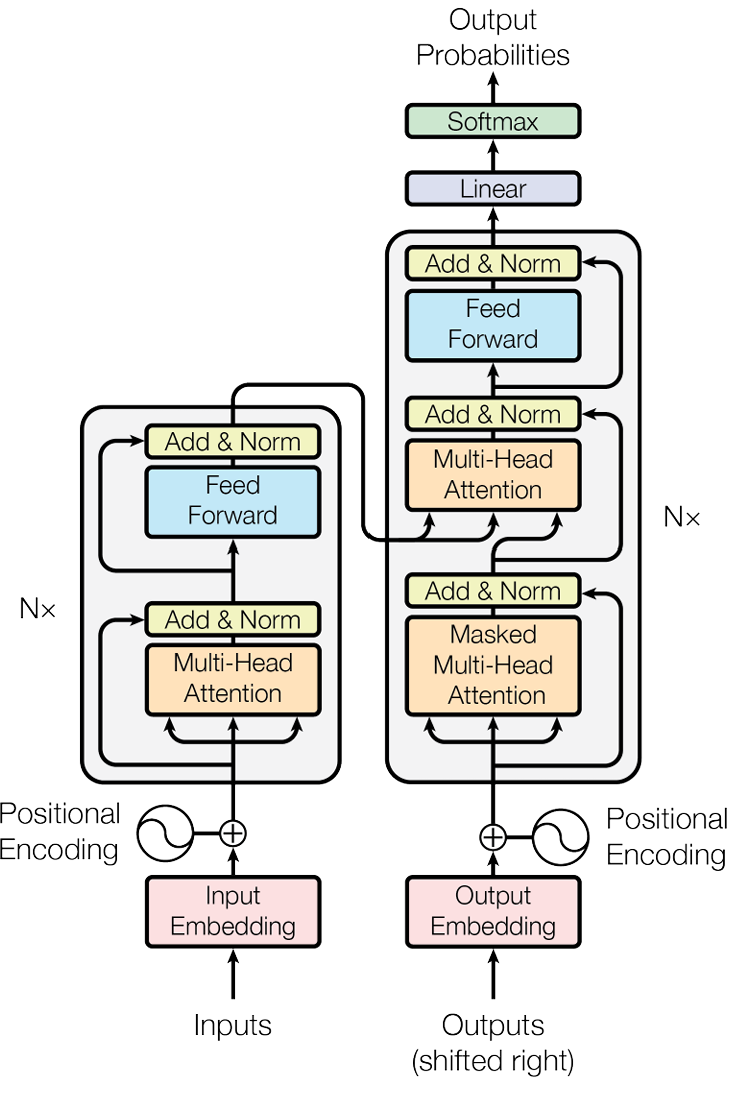
\includegraphics[width=0.3\textwidth]{figuras/capitulo1/transformer_architecture.png}
\caption{Arquitectura básica de un Transformer.}
\label{fig:transformer_architecture}
\end{figure}

\subsection{Transición de PLMs a LLMs}
La transición de los modelos de lenguaje preentrenados (PLMs) a los modelos grandes del lenguaje (LLMs) se caracterizó por un aumento significativo en el tamaño de los modelos y la cantidad de datos de entrenamiento. Modelos como GPT-3, con 175 mil millones de parámetros, demostraron que el escalado de los modelos y los datos de entrenamiento puede llevar a mejoras drásticas en el rendimiento en una amplia gama de tareas de NLP. Los LLMs han mostrado capacidades sorprendentes en tareas de zero-shot y few-shot learning, donde pueden realizar tareas no vistas durante el entrenamiento con poca o ninguna adaptación adicional. La Figura \ref{fig:llm_evolution} muestra la evolución cronológica de los principales LLMs.

\begin{figure}[h]
\centering
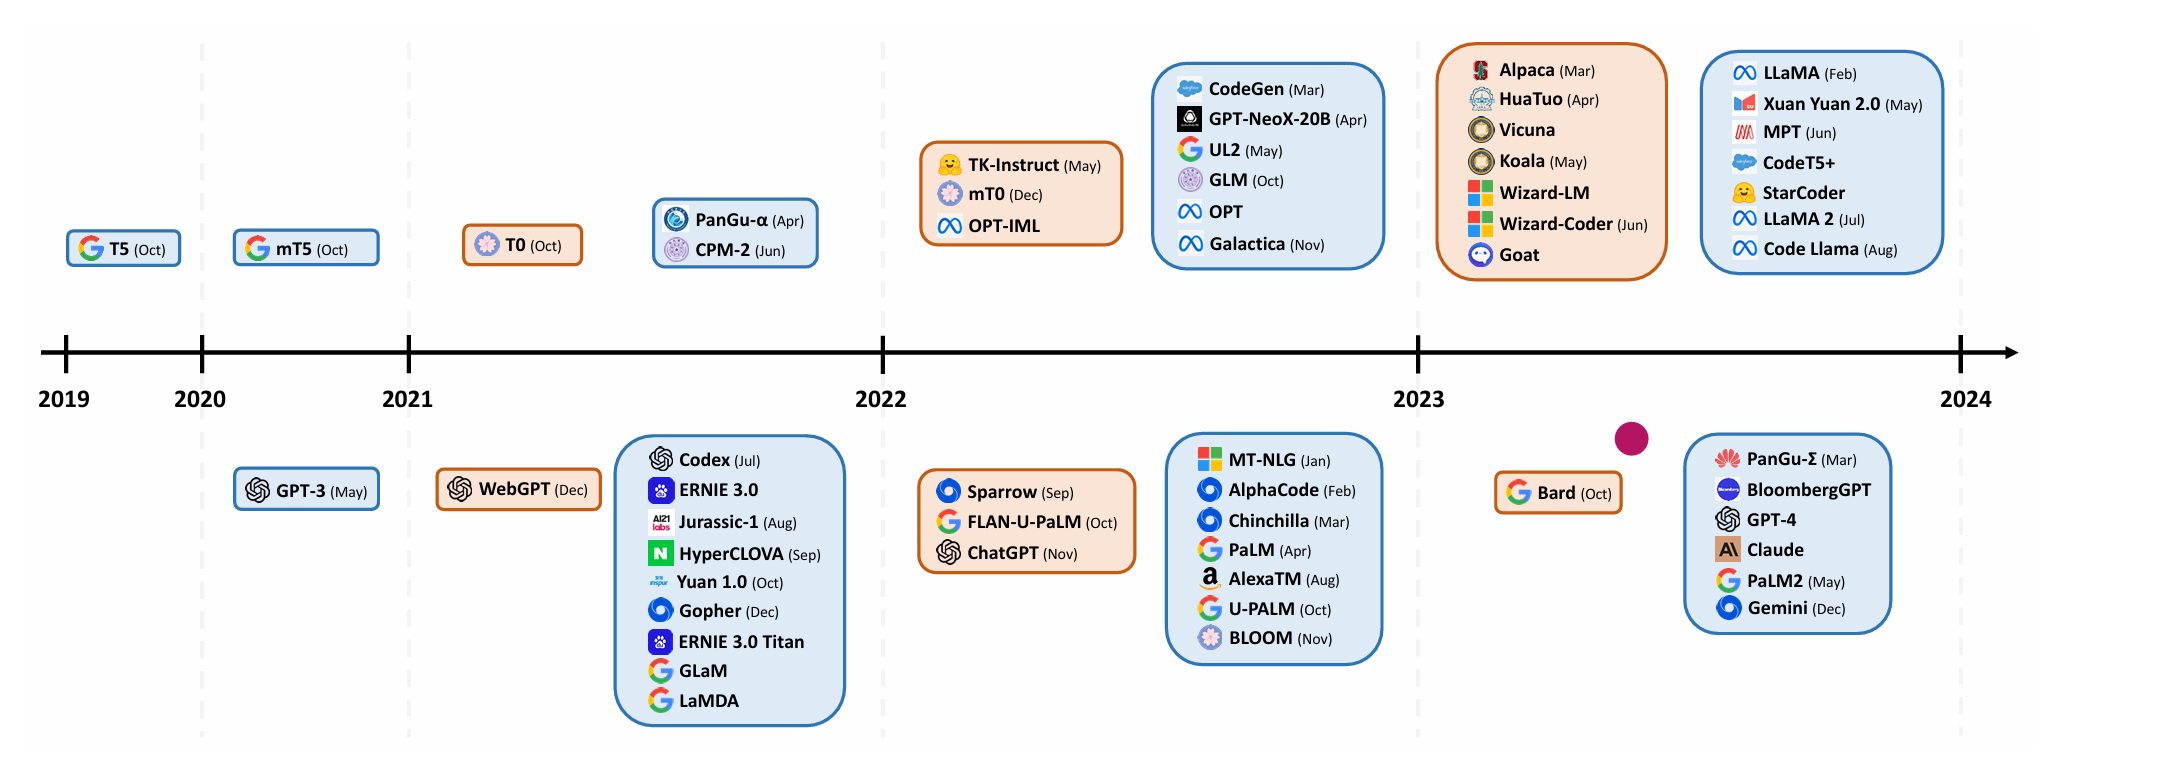
\includegraphics[width=0.85\textwidth]{figuras/capitulo1/llm_evolution.png}
\caption{Evolución cronológica de los principales LLMs.}
\label{fig:llm_evolution}
\end{figure}


\section{Arquitecturas y Modelos Importantes}
En los últimos años, los Modelos grandes del lenguaje (LLMs) han experimentado avances significativos, lo que ha resultado en la creación de arquitecturas y modelos innovadores. Estos modelos no solo han mejorado en términos de capacidad y precisión, sino que también han introducido nuevas formas de abordar problemas complejos en el procesamiento de lenguaje natural. A continuación, se presentan algunas de las arquitecturas históricas y modelos más importantes en el ámbito de los LLMs.

\subsection{T5 (Text-to-Text Transfer Transformer)}
El modelo T5, desarrollado por Google, es un modelo de codificador-decodificador que trata todas las tareas de procesamiento de lenguaje natural (NLP) como problemas de generación de texto. Esto significa que convierte todas las tareas de entrada en una estructura de texto a texto, lo que permite un enfoque unificado para diversas tareas de NLP.

\begin{figure}[h]
\centering
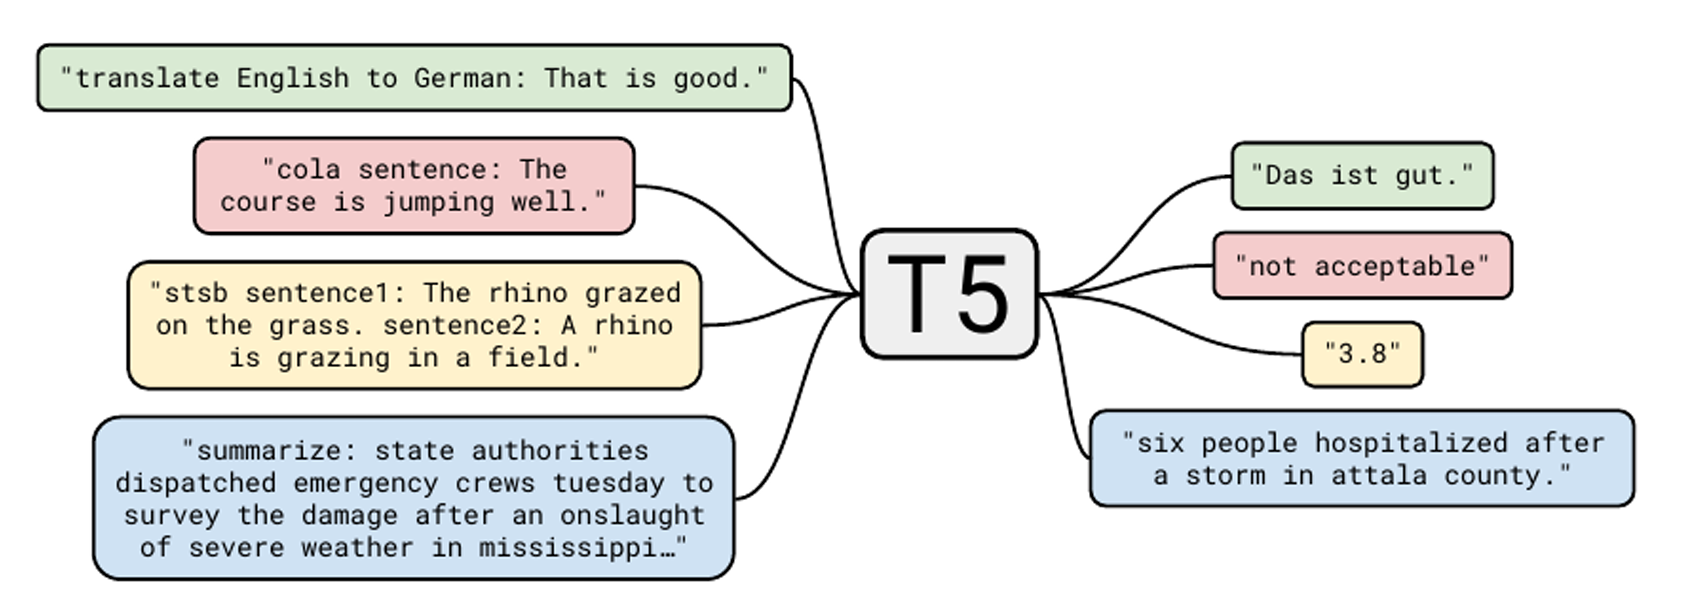
\includegraphics[width=0.85\textwidth]{figuras/capitulo1/t5.png}
\caption{Ejemplo unificado de formación texto a texto, imagen origen de \citep{raffel2020exploring}}
\label{fig:llm_evolution}
\end{figure}

\subsection{BERT (Bidirectional Encoder Representations from Transformers)}
BERT, desarrollado por Google \citep{devlin2018bert}, es un modelo basado en transformers que se entrena utilizando un objetivo de modelado de lenguaje enmascarado, donde se predicen tokens enmascarados dentro de una secuencia utilizando el contexto bidireccional de la secuencia completa. Este enfoque permite a BERT capturar relaciones más complejas y contextuales en el texto en comparación con los modelos unidireccionales. La capacidad de BERT para ser finetuneado de manera eficiente sin requerir modificaciones sustanciales en la arquitectura específica de cada tarea ha contribuido significativamente a su adopción y éxito en múltiples dominios de NLP.

\subsection{mT5 (Multilingual T5)}
mT5 es una variante multilingüe del modelo T5, entrenada en el dataset mC4 que abarca 101 idiomas. Este modelo utiliza un vocabulario más amplio de 250,000 tokens para cubrir múltiples lenguajes. Para evitar el sobreajuste o subajuste en un idioma específico, mT5 emplea un procedimiento de muestreo de datos que selecciona muestras de todos los idiomas. Además, durante el afinamiento para tareas específicas utilizando datos en inglés, el modelo puede generar salidas correctas en otros idiomas.

\subsection{GPT-3 (Generative Pre-trained Transformer 3)}
GPT-3, desarrollado por OpenAI, es uno de los modelos de lenguaje más grandes y avanzados hasta la fecha, con 175 mil millones de parámetros. GPT-3 utiliza una arquitectura de transformers similar a GPT-2 pero con atención densa y dispersa en las capas del transformer. Este modelo demostró que el escalado masivo del tamaño del modelo y los datos de entrenamiento puede llevar a mejoras significativas en el rendimiento en una amplia gama de tareas de NLP. GPT-3 es especialmente conocido por su capacidad de realizar tareas en configuraciones de zero-shot, few-shot y one-shot learning, proporcionando respuestas coherentes y contextualmente relevantes. \hfill \break

\begin{figure}[h]
\centering
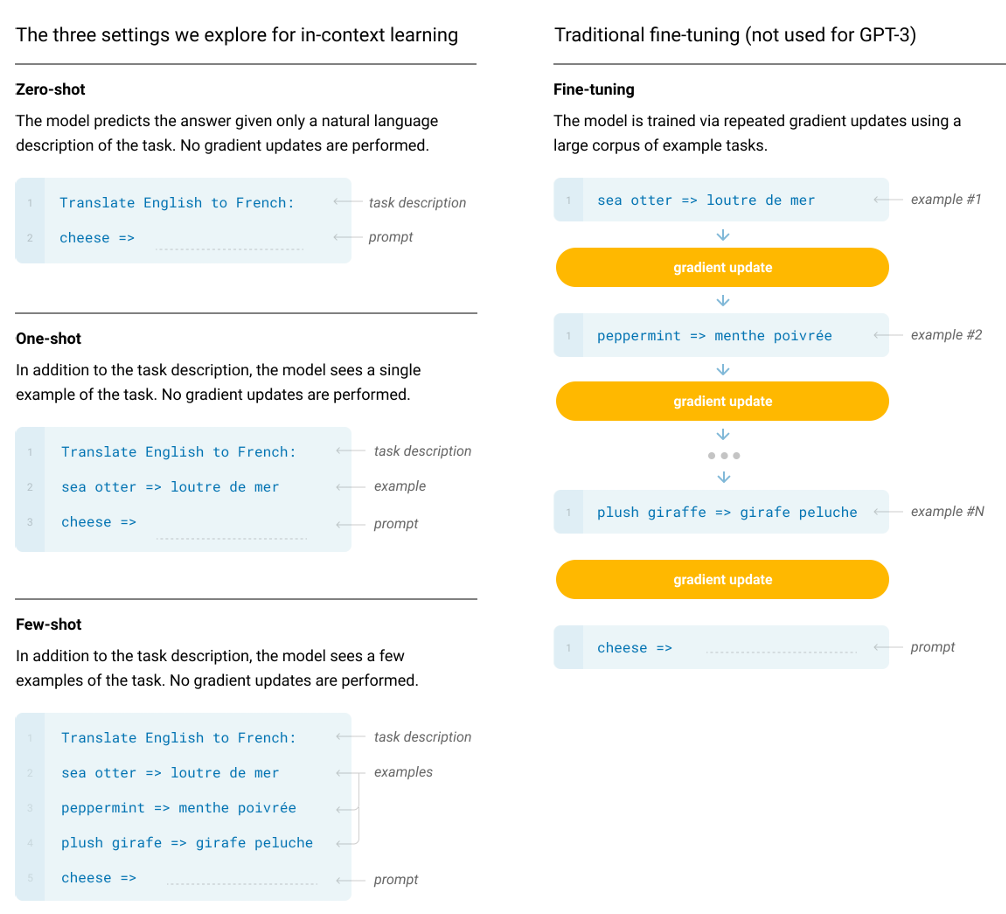
\includegraphics[width=0.6\textwidth]{figuras/capitulo1/gpt3.png}
\caption{Zero-shot, one-shot y few-shot contrastado con finetunning tradicional. Imagen origen de \citep{brown2020language}}
\label{fig:llm_evolution}
\end{figure}


Entre todos estos avances han llegado infinidad de modelos y arquitecturas que han presentado avances significativos en el ámbito del NLP creando un antes y un después en la figura de los LLMs, véase en la figura \ref{fig:llm_evolution}. Desde modelos abiertos como Llama (meta) y Mistral hasta modelos propietarios como GPT4 (OpenAI) o Claude (Anthropic) en sus diferentes versiones.


\section{Aplicaciones de los LLMs}
\subsection{Generación de Texto}

\subsection{Resumen Automático}

\subsection{Traducción Automática}

\subsection{Interacción Conversacional}

\subsection{Respuesta a Preguntas}


\section{Desafíos y Futuras Direcciones}
\subsection{Costos Computacionales y Energéticos}

\subsection{Generalización y Adaptación de Dominios}

\subsection{Seguridad y Ética}

\subsection{Privacidad y Datos Sensibles}


\cleardoublepage

\chapter{Retrieval Augmented Generation (RAGs)}
\label{Retrieval Augmented Generation (RAGs)}
% INTRODUCCIÓN

\cleardoublepage

\chapter{Estrategias de chunkerización para LLMs}
\label{Estrategias de chunkerización}

\section{Introducción}
La chunkerización en el ámbito de los modelos de lenguaje de gran escala (LLM) se refiere al proceso de dividir textos extensos en segmentos más manejables, conocidos como \textit{chunks}. Esta técnica es fundamental para mejorar la gestión y el procesamiento de grandes volúmenes de información en aplicaciones de inteligencia artificial que utilizan modelos de lenguaje para entender y generar texto humano.

\textbf{Necesidad de la Chunkerización:} Los modelos de lenguaje, son inherentemente limitados por la cantidad de texto que pueden procesar en una sola instancia debido a restricciones de memoria y capacidad de cálculo. Al descomponer los textos en chunks más pequeños, se facilita que el modelo maneje datos extensos de manera eficiente, permitiendo una evaluación más rápida y precisa.

\textbf{Objetivos de la Chunkerización:} El principal objetivo de la chunkerización es maximizar la relevancia y la precisión del texto procesado. Al dividir el contenido en partes significativas y manejables, se busca preservar la coherencia semántica sin sobrecargar el modelo. Además, esta estrategia es crucial para la indexación efectiva de contenidos en bases de datos vectoriales, lo que mejora la recuperación y relevancia de los resultados en consultas específicas.

\textbf{Retos de la Chunkerización:} A pesar de sus beneficios, la chunkerización presenta varios desafíos. El más significativo es determinar el tamaño óptimo de cada chunk. Si los chunks son demasiado pequeños, pueden perder contexto necesario para una comprensión completa; si son demasiado grandes, pueden exceder las capacidades de procesamiento del modelo y diluir la relevancia del contenido. Otro reto es la selección de los puntos de corte dentro del texto, que debe hacerse de manera que se preserve la integridad del contenido semántico.

La chunkerización es un proceso esencial que requiere un cuidadoso equilibrio entre tamaño de chunk, preservación del contexto y capacidades del modelo. En las siguientes secciones, exploraremos diferentes estrategias y métodos de chunkerización, evaluando sus ventajas y limitaciones en diversos contextos de aplicación.

\section{Consideraciones sobre la Chunkerización}

Al desarrollar una estrategia de chunkerización eficaz, es crucial considerar varios aspectos que influirán en el rendimiento y la eficacia del modelo de lenguaje. A continuación, se detallan algunas de las consideraciones más importantes:

\subsection{Naturaleza del Contenido}
El tipo de contenido que se está indexando es determinante en la selección de la estrategia de chunkerización. Por ejemplo, documentos largos como artículos o libros pueden requerir un enfoque diferente en comparación con contenidos más breves como tuits o mensajes instantáneos. Esta distinción afecta tanto la elección del modelo para crear los embeddings como la estrategia de chunkerización a aplicar.

\subsection{Modelo y Tamaño Óptimo del Chunk}
Dependiendo del modelo utilizado para crear los embeddings, existirán tamaños de chunk en los que el modelo desempeñará mejor. Por ejemplo, algunos modelos están optimizados para trabajar con frases individuales, mientras que otros pueden manejar mejor segmentos de texto más largos. Identificar el tamaño de chunk que maximiza la calidad de los embeddings es crucial para el éxito de la estrategia de chunkerización.

\subsection{Complejidad y Longitud de las Consultas de Usuario}
Las expectativas sobre la longitud y complejidad de las consultas de los usuarios deben guiar la manera en que se chunkeriza el contenido. Si las consultas suelen ser cortas y específicas, es posible que se prefiera chunkerizar el contenido en segmentos más pequeños para reflejar esta especificidad. En cambio, consultas más largas y complejas podrían beneficiarse de chunks más grandes que proporcionen un contexto más amplio.

\subsection{Uso de los Resultados Recuperados}
El propósito final de los chunks recuperados también juega un papel crucial. Dependiendo de si los resultados serán utilizados para búsqueda semántica, respuesta a preguntas, resumen, o cualquier otro fin, la estrategia de chunkerización podría variar para optimizar la relevancia y utilidad de la información recuperada.

\subsection{Limitaciones Técnicas}
Las limitaciones técnicas, como el número máximo de tokens que el modelo puede procesar en una sola instancia o las restricciones de memoria, son críticas para definir el tamaño de los chunks. Estas limitaciones no solo afectan cómo se chunkeriza el contenido sino también cómo se procesa posteriormente en el modelo.

Estas consideraciones son fundamentales para desarrollar una estrategia de chunkerización que no solo sea eficiente sino también efectiva en términos de mejorar la relevancia y precisión de las respuestas del modelo.

\section{Estrategias de Chunkerización}

La chunkerización puede implementarse de diversas maneras, cada una con sus propios beneficios y desafíos. A continuación, exploramos algunas de las estrategias más comunes y cómo pueden optimizarse según diferentes necesidades y contextos.

\subsection{Chunkerización de Tamaño Fijo}

Esta estrategia consiste en dividir el texto en segmentos de un tamaño predeterminado, medido en número de tokens o carácteres. La principal ventaja de este método es su simplicidad y facilidad de implementación, ya que no requiere un análisis profundo del contenido. Sin embargo, un desafío significativo es que puede cortar frases a la mitad, perdiendo contexto o generando chunks que carecen de sentido por sí solos. Para mitigar esto, se puede optar por incluir una superposición entre los chunks, donde el final de un chunk se superpone con el inicio del siguiente, ayudando a preservar el contexto (overload).

\begin{figure}[h]
\centering
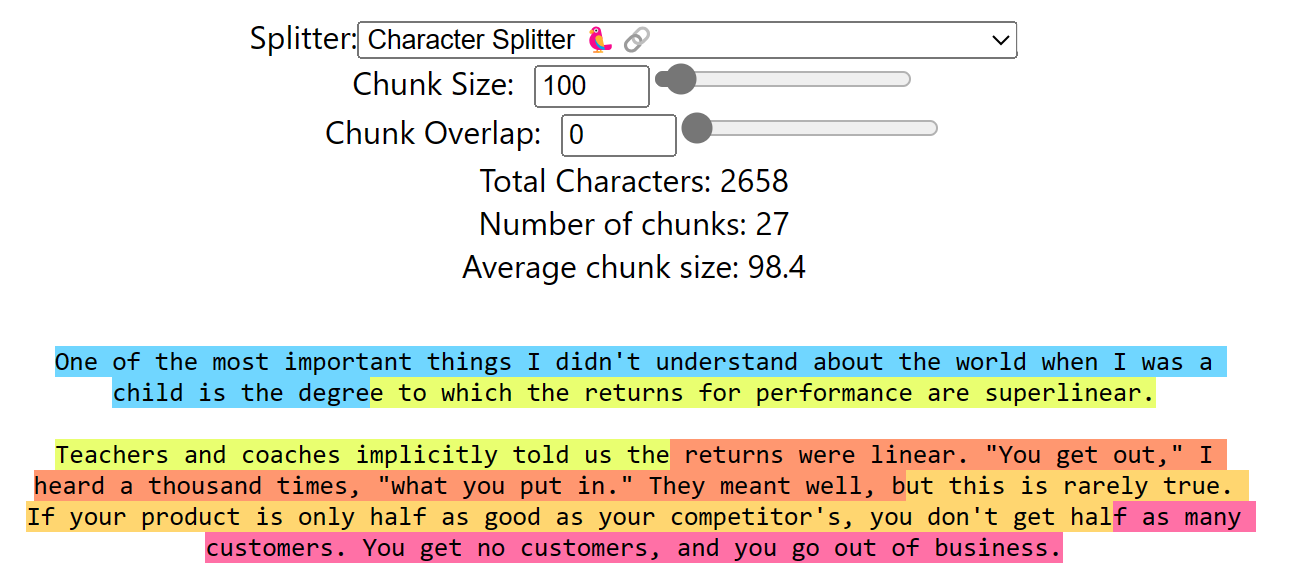
\includegraphics[width=0.8\textwidth]{figuras/capitulo4/character_splitter_100_0.png}
\caption{Ejemplo de chunkerización tamaño fijo sin overload}
\label{fig:imagen_fijo}
\end{figure}

\begin{figure}[h]
\centering
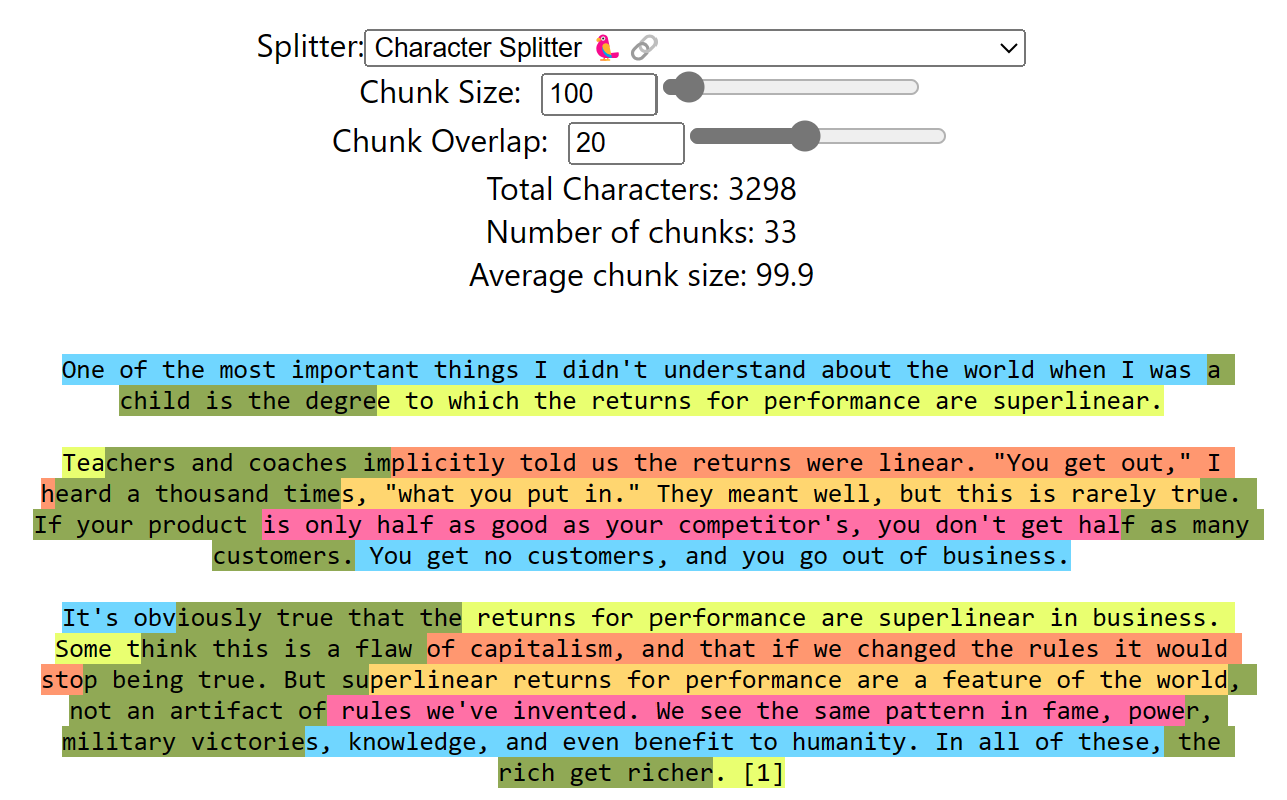
\includegraphics[width=0.8\textwidth]{figuras/capitulo4/character_splitter_100_20.png}
\caption{Ejemplo de chunkerización tamaño fijo con overload}
\label{fig:imagen_fijo_overload}
\end{figure}

\subsection{Chunkerización Consciente del Contenido}

A diferencia de la chunkerización de tamaño fijo, este método tiene en cuenta el contenido textual para determinar los puntos de corte. La chunkerización consciente del contenido puede basarse en la detección de fronteras naturales en el texto, como finales de oraciones o párrafos, asegurando que cada segmento contenga una unidad completa de información. Esto ayuda a mantener la coherencia semántica de los chunks, haciendo que cada uno sea significativo por sí mismo y mejore la calidad de las incrustaciones generadas por el modelo. Este método es particularmente útil en documentos con una estructura clara y bien definida, como artículos académicos o reportes técnicos.

\subsection{Chunkerización Recursiva}

Este enfoque implica un proceso iterativo y jerárquico de dividir el texto en chunks. Inicialmente, el texto se divide utilizando un criterio de separación amplio, y si los chunks resultantes aún son demasiado grandes o no cumplen con ciertos criterios, el proceso se repite en cada chunk hasta alcanzar el tamaño o la estructura deseada. La chunkerización recursiva es útil en textos largos y complejos donde los niveles múltiples de división permiten manejar mejor la diversidad y complejidad del contenido.

\begin{figure}[!h]
\centering
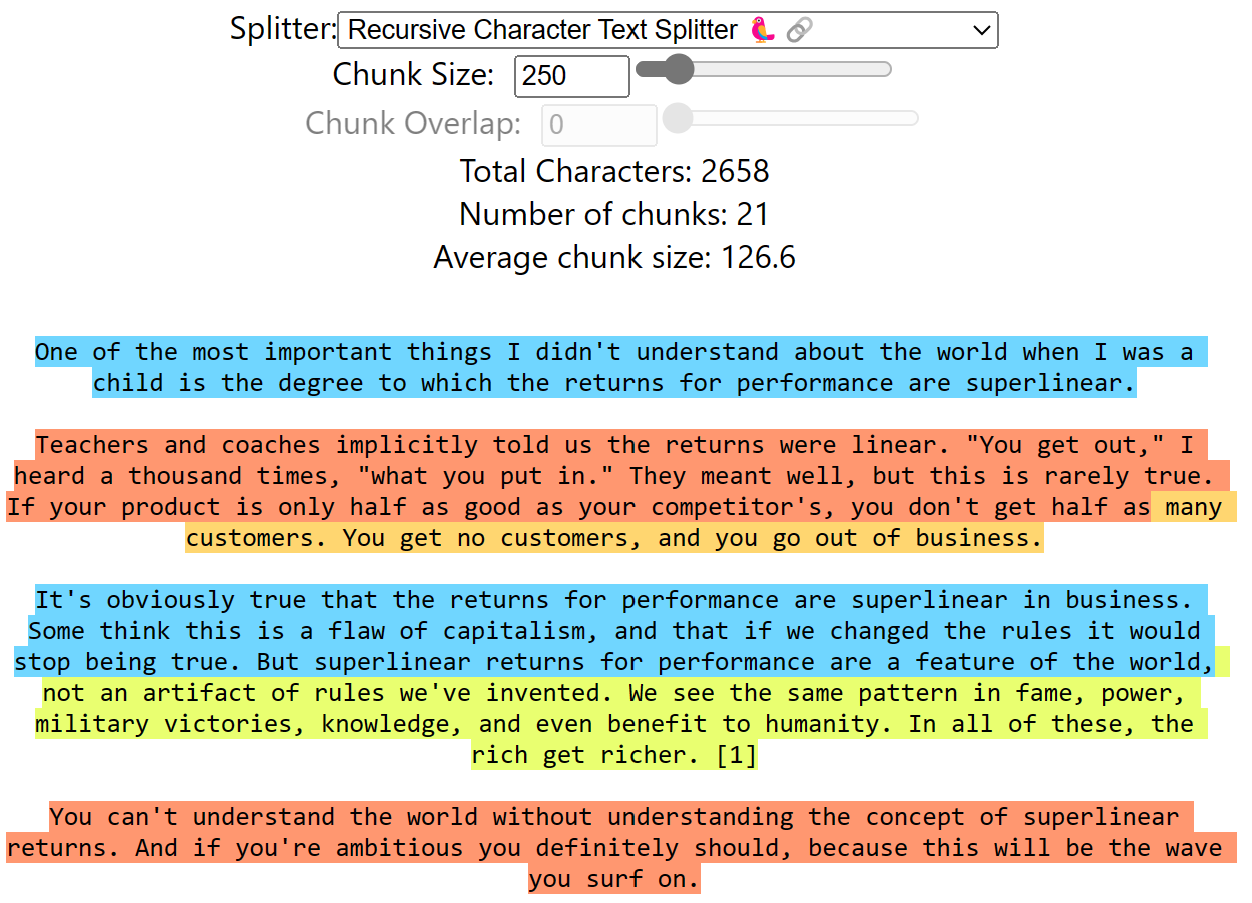
\includegraphics[width=0.8\textwidth]{figuras/capitulo4/recursive_character_splitter_250_0.png}
\caption{Ejemplo de chunkerización recursiva}
\label{fig:imagen_recursiva}
\end{figure}

\subsection{Chunkerización Especializada}

Esta estrategia se adapta a formatos de contenido específicos que requieren un tratamiento particular, como puede ser el caso de textos en Markdown o LaTeX. La chunkerización especializada reconoce y respeta la estructura y sintaxis propias de estos formatos, asegurando que los chunks resultantes conserven la integridad y funcionalidad del texto original. Por ejemplo, en un documento LaTeX, los chunks podrían definirse para encapsular secciones completas o subsecciones, preservando las etiquetas y comandos propios del formato.

Cada una de estas estrategias tiene sus propias fortalezas y puede ser más adecuada para diferentes tipos de textos y aplicaciones. La elección de una estrategia de chunkerización debe basarse en una evaluación cuidadosa de los requisitos del proyecto, la naturaleza del contenido y los objetivos específicos del sistema de procesamiento de lenguaje natural.

\begin{figure}[!h]
\centering
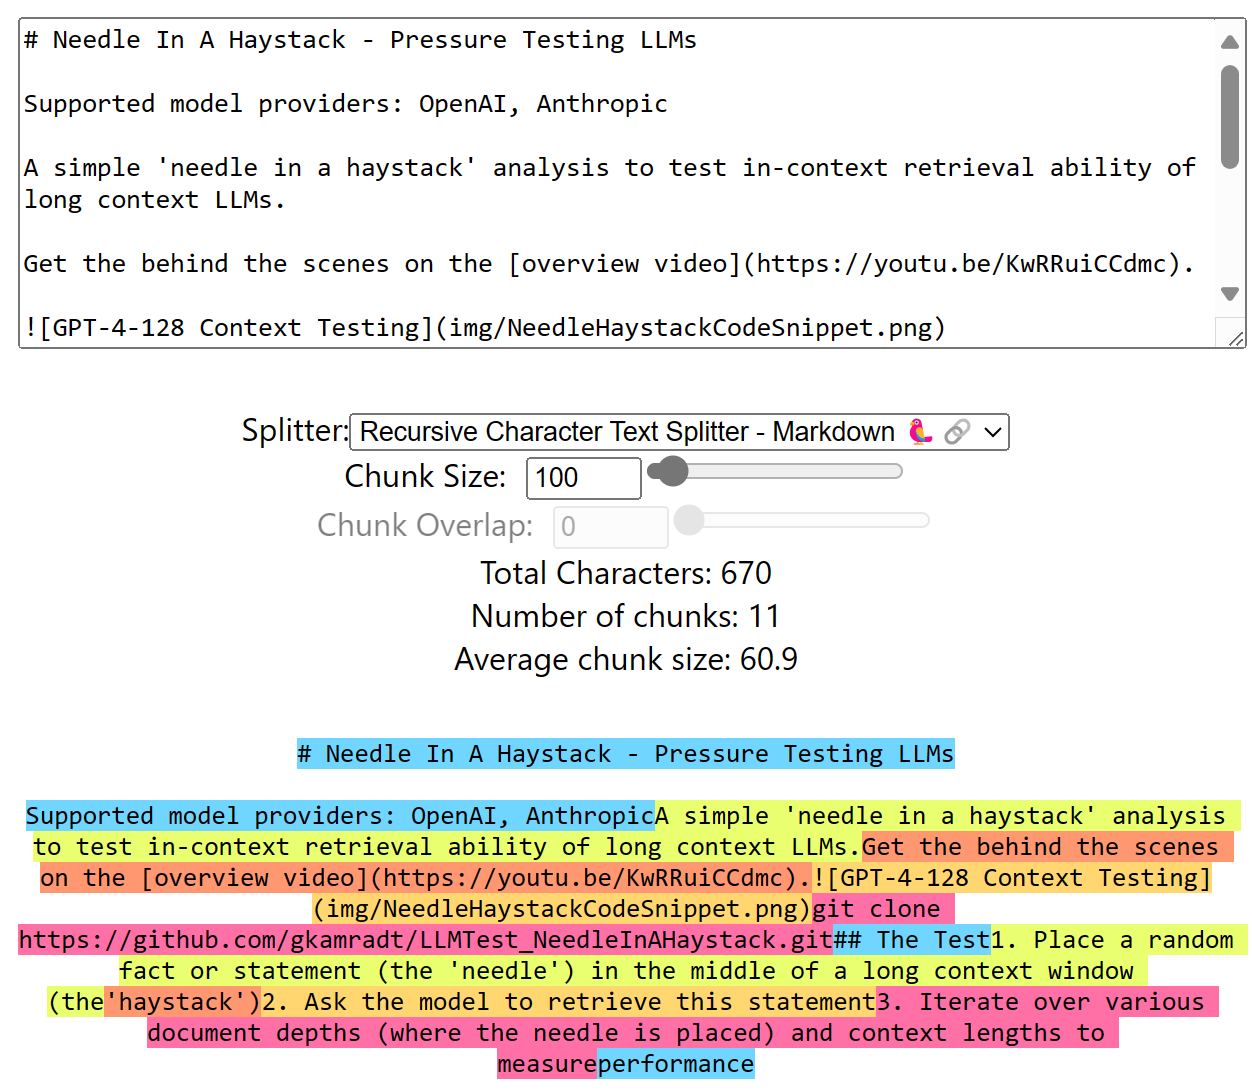
\includegraphics[width=0.8\textwidth]{figuras/capitulo4/character_md_100.png}
\caption{Ejemplo de chunkerización Especializada}
\label{fig:imagen_chunk_md}
\end{figure}

\subsection{Chunkerización Semántica}

La chunkerización semántica es una técnica avanzada que divide el texto en unidades basadas en la relevancia semántica, utilizando modelos de creación de embeddings para evaluar la similitud entre segmentos de texto.

\subsubsection{Implementación y Ventajas}
Esta estrategia se implementa mediante la transformación de texto en representaciones vectoriales y el cálculo de su similitud, agrupando segmentos similares. Es especialmente útil para mantener la coherencia del contenido en tareas de recuperación de información y análisis de texto.

\subsubsection{Desafíos y Aplicaciones}
A pesar de su efectividad, enfrenta desafíos como la alta demanda computacional y la dificultad en determinar umbrales de similitud óptimos. Su aplicación es ideal en sistemas de búsqueda semántica y en el análisis de textos complejos en contextos académicos o de investigación.


\section{Conclusiones}
La chunkerización es fundamental para mejorar la eficiencia y precisión en aplicaciones relacionadas con LLM. No existe una solución única para todos los casos, por lo que es crucial evaluar cada situación individualmente para encontrar la estrategia más efectiva.

% INTRODUCCIÓN

\cleardoublepage

\chapter{Retrievers}

\section{Introducción}

Habiendo introducido los conceptos fundamentales de los Modelos de Lenguaje a Gran Escala (LLMs) y los RAG en los capítulos anteriores, ahora nos centramos en uno de los componentes críticos que potencian los sistemas RAG: los \textit{retrievers}. Este concepto es esencial para la creación de un RAG sobre un LLM, permitiéndole acceder a información actualizada y relevante más allá de su entrenamiento inicial.

En este capítulo, exploraremos los diferentes tipos de \textit{retrievers}, cómo se integran en los sistemas RAG y las distintas metodologías para su implementación. Discutiremos desde los simples \textit{retrievers} basados en bases de datos vectoriales hasta complejas configuraciones que involucran múltiples métodos de recuperación de información.

\section{Fundamentos de los Retrievers}

\subsection{Definición y Función}

Un \textit{retriever} es una herramienta que busca y recupera información relevante de un conjunto de datos grande y posiblemente no estructurado. En el contexto de RAG, un \textit{retriever} actúa como el puente entre la pregunta del usuario y la base de conocimientos o información almacenada. La eficacia de un \textit{retriever} es crucial, ya que determina la calidad y la relevancia de la información que se utiliza para generar respuestas.

\subsection{Rol en RAG}

Como se puede ver en la figura \ref{fig:retriever}, en un sistema RAG, el retriever selecciona fragmentos de texto o documentos que son potencialmente útiles para responder a una consulta específica. Estos documentos se pasan luego a un modelo de lenguaje, que integra esta información para generar una respuesta coherente y contextualmente rica. Esta capacidad de incorporar información dinámica de diversas fuentes externas distingue a los RAGs de los modelos de lenguaje tradicionales que dependen únicamente de lo que han aprendido durante su entrenamiento inicial.

\begin{figure}[h]
\centering
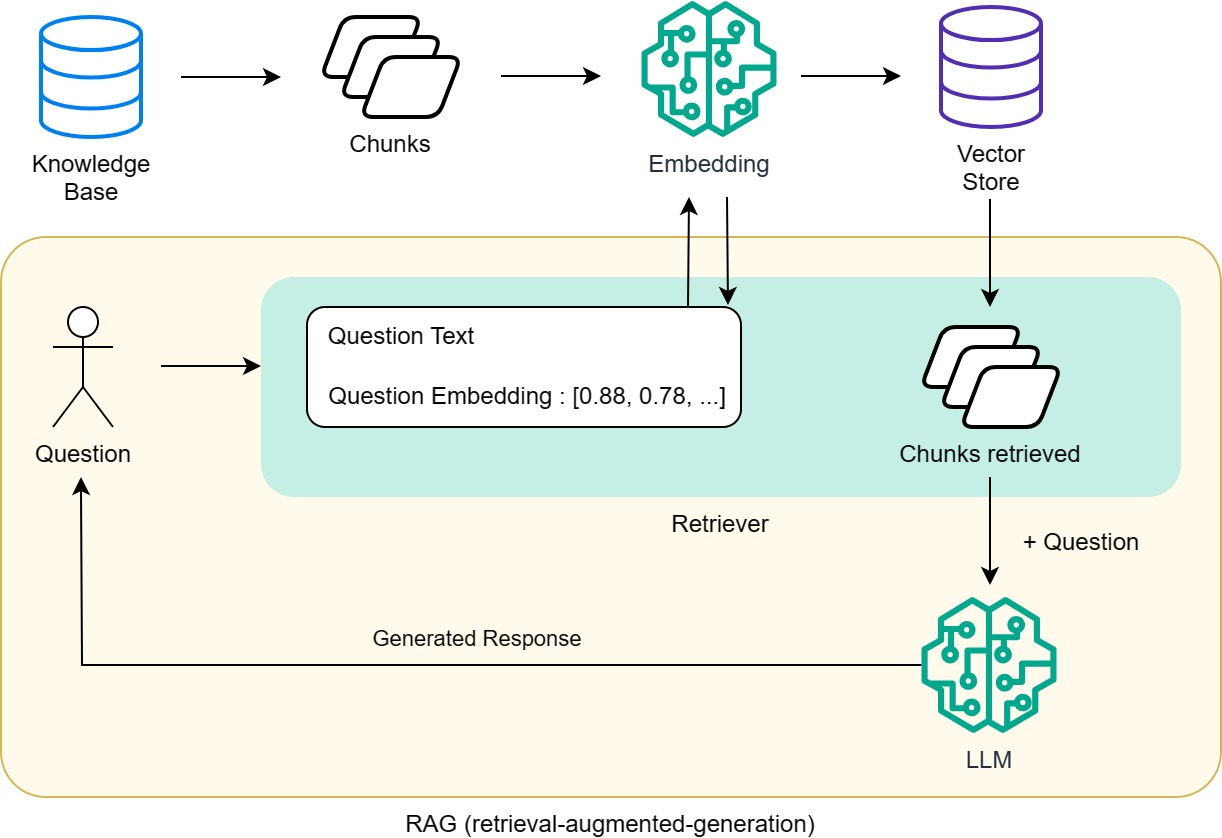
\includegraphics[width=0.8\textwidth]{figuras/capitulo5/retriever.jpg}
\caption{Esquema de un RAG}
\label{fig:retriever}
\end{figure}

\section{Tipos de Retrievers Tradicionales}

Los retrievers se clasifican principalmente en tres tipos, cada uno con sus propias técnicas y aplicaciones preferidas en el procesamiento de consultas y la recuperación de información. Estos son los retrievers \textit{sparse}, \textit{dense} e \textit{hybrid}.

\subsection{Retrievers Sparse}

Los retrievers \textit{sparse} utilizan métodos basados en coincidencia de términos para recuperar documentos. Estos métodos, como TF-IDF (Frequency-Inverse Document Frequency) y BM25, analizan la frecuencia de las palabras en documentos para determinar su relevancia con respecto a una consulta. La principal ventaja de los retrievers sparse es su eficiencia y rapidez, lo que los hace adecuados para grandes volúmenes de datos donde la relevancia se puede medir por la presencia de palabras clave específicas. \citep{lewis2020retrieval}

Estos retrievers son particularmente útiles en situaciones donde las consultas son directas y las palabras clave bien definidas son suficientes para recuperar información relevante. Sin embargo, pueden no ser efectivos en contextos donde la semántica de la consulta es más importante que las palabras específicas utilizadas.

\subsection{Retrievers Dense}

Por otro lado, los retrievers \textit{dense} emplean modelos de vectorización (embeddings) para representar tanto las consultas como los documentos como vectores densos en un espacio vectorial continuo. Estos modelos capturan la semántica de las palabras y las frases, permitiendo una recuperación más efectiva en casos donde las consultas y los documentos no comparten términos exactos pero están relacionados en contexto y significado. \citep{lewis2020retrieval}

Los retrievers dense son esenciales para aplicaciones donde la relevancia semántica entre la consulta y los documentos es más crítica que la coincidencia exacta de palabras. Su capacidad para entender y procesar el lenguaje de manera más natural los hace muy valiosos en sistemas RAG modernos. Estos retrievers son muy dependientes del modelo de vectorización usado.

\subsection{Retrievers Hybrid}

Finalmente, los retrievers \textit{hybrid} combinan las técnicas de los retrievers sparse y dense para aprovechar las ventajas de ambos. Este enfoque permite una recuperación inicial rápida de documentos potencialmente relevantes utilizando métodos sparse, seguida de un refinamiento más detallado y semánticamente rico con técnicas dense.

Los retrievers hybrid ofrecen un equilibrio entre eficiencia y profundidad semántica, lo que los hace ideales para sistemas RAG que requieren tanto precisión en la recuperación de información relevante como la capacidad de manejar grandes volúmenes de datos.

Cada tipo de retriever tiene su lugar en el ecosistema de los RAG, y la elección de uno sobre otro depende en gran medida de las necesidades específicas del sistema y las características de las consultas y los conjuntos de datos utilizados.

\section{Retrievers Avanzados}

Dada la evolución constante de los sistemas RAG y la necesidad de integrar información más específica y contextual, la comunidad ha estado desarrollando diferentes retrievers que tienen sentido en determinados contextos. Estos retrievers utilizan técnicas sofisticadas para mejorar la precisión y la relevancia de la información recuperada. Aquí exploramos varios enfoques que se recopilan en la web de langchain \citep{langchainretrievers}.

\subsection{Documento Matriz (Parent Document)}

Este tipo de retriever es ideal cuando los documentos contienen numerosos fragmentos de información distintos que se benefician de ser indexados individualmente, pero que es preferible recuperar juntos. El proceso involucra la indexación de múltiples fragmentos o trozos de cada documento. Luego, estos fragmentos se buscan en el espacio de vectores (embeddings) para identificar aquellos que son más similares entre sí, pero en lugar de recuperar solo los fragmentos individuales, se recupera y devuelve el documento completo al que pertenecen. Esta metodología asegura que toda la información contextual relacionada esté disponible para generar respuestas más completas y detalladas.

\subsubsection{Multi Vector}

Este retriever es especialmente útil cuando es posible extraer de los documentos información que se considera relevante para indexar (a parte del texto en sí). El proceso implica la creación de múltiples vectores para cada documento. Cada vector puede ser generado de diversas maneras, incluyendo, por ejemplo, resúmenes del texto, preguntas hipotéticas, descripciones de imágenes o tablas, etc. 
Esta técnica permite una representación más rica de los documentos, facilitando una recuperación más precisa y alineada con las necesidades específicas del retriever.


\subsection{Consulta Autónoma (Self Query)}

Utiliza un LLM para transformar la entrada del usuario en dos componentes principales: una cadena que se busca semánticamente y un filtro de metadatos que acompaña la consulta. Este método es particularmente valioso porque muchas veces las preguntas están relacionadas con los metadatos de los documentos, no con su contenido textual directo. La capacidad de enfocar la búsqueda en metadatos permite recuperar información que es más relevante para la intención específica del usuario, mejorando así la precisión y utilidad de las respuestas generadas. Este tipo de retriever es especialmente útil cuando las preguntas de los usuarios se responden mejor recuperando documentos basados en metadatos en lugar de en similitudes textuales directas

\begin{figure}[h]
\centering
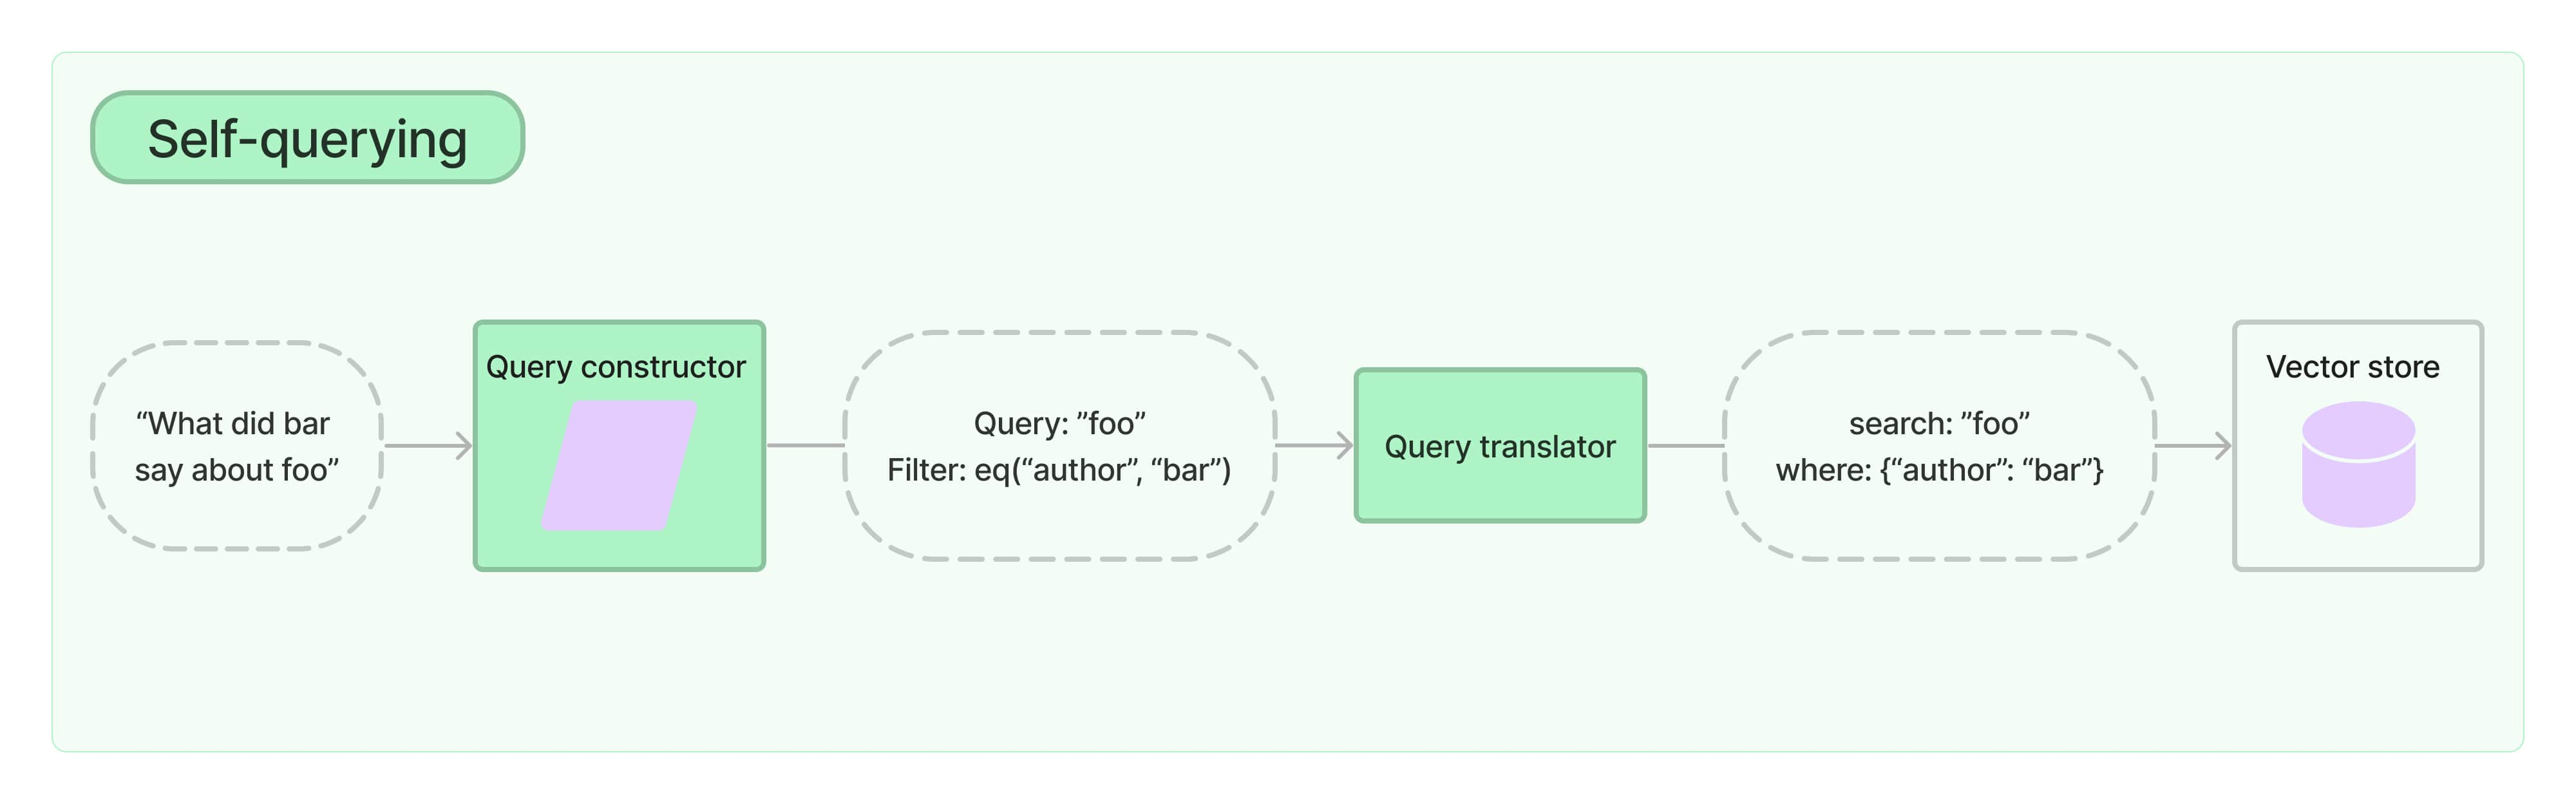
\includegraphics[width=0.8\textwidth]{figuras/capitulo5/self_query.jpg}
\caption{Esquema de un Self Query retriever \citep{langchainretrievers}}
\label{fig:retrieverselfquery}
\end{figure}


\subsubsection{Compresión Contextual}

Uno de los desafíos en la recuperación de documentos es que generalmente no se conocen las consultas específicas que enfrentará el sistema de almacenamiento de documentos cuando se ingieren datos en el sistema. Esto significa que la información más relevante para una consulta puede estar enterrada en un documento con mucho texto irrelevante. Pasar ese documento completo a través de la aplicación puede llevar a llamadas más costosas al LLM y a respuestas de menor calidad.

La compresión contextual está diseñada para solucionar esto. En lugar de devolver inmediatamente los documentos recuperados tal como están, se pueden comprimir utilizando el contexto de la consulta dada, de modo que solo se devuelva la información relevante.


\subsection{Time-Weighted Vectorstore}

Optimiza la recuperación basándose tanto en la similitud semántica como en la fechateams del documento. Es ideal para aplicaciones donde la información más actual es crucial, como en el seguimiento de noticias o tendencias del mercado.

\subsection{Multi-Query Retriever}

Genera múltiples consultas a partir de una inicial para abordar consultas complejas que requieren información sobre varios temas. Luego, recupera documentos para cada una de estas consultas, lo que garantiza una respuesta exhaustiva y detallada. Es muy útil cuando las preguntas van a tratar sobre varios temas y temas no relacionados.

\subsection{Long-Context Reorder}

Es especialmente útil en modelos que enfrentan degradaciones de rendimiento cuando deben acceder a información relevante en medio de contextos extensos. Este tipo de retriever reordena los documentos recuperados para optimizar la atención del modelo a la información más pertinente, colocando los documentos más relevantes al principio y al final, mientras que los menos relevantes quedan en el medio.
El "Long Context Reorder" utiliza un enfoque específico conocido como "Lost in the middle" para contrarrestar el problema de que los modelos ignoren documentos importantes simplemente porque aparecen en posiciones menos destacadas dentro de un conjunto de datos grande. \citep{liu2023lost}

Estos retrievers avanzados representan un conjunto diverso de herramientas diseñadas para mejorar la eficiencia y efectividad de los sistemas RAG, facilitando respuestas más precisas y contextuales en una amplia variedad de aplicaciones.

\section{Conclusión}

A lo largo de este capítulo, hemos explorado en profundidad los diversos tipos de \textit{retrievers} que potencian los sistemas de RAG. Hemos visto cómo los \textit{retrievers} no solo facilitan la recuperación de información relevante y actualizada, sino que también optimizan la eficiencia del procesamiento y la precisión de las respuestas generadas por los LLMs. La implementación adecuada de estos \textit{retrievers} puede marcar una diferencia significativa en la capacidad de un sistema RAG para proporcionar respuestas precisas, contextuales y de alta calidad.

Este capítulo también ha subrayado la importancia de elegir el tipo correcto de \textit{retriever} según las necesidades específicas del sistema y del dominio de aplicación. Con las tecnologías emergentes y los desarrollos continuos en el campo de la inteligencia artificial, es probable que veamos aún más innovaciones en los métodos de recuperación, lo que a su vez podría ampliar aún más las capacidades y aplicaciones de los RAGs.

En resumen, los \textit{retrievers} son componentes cruciales que no solo enriquecen la funcionalidad de los sistemas basados en LLMs mediante la incorporación de conocimientos actualizados y contextualmente relevantes, sino que también representan un área de investigación activa y en evolución que continuará influyendo en el futuro de la generación de lenguaje y la recuperación de información.






% INTRODUCCIÓN

\cleardoublepage

\chapter{Sistema RAG aplicado a la Constitución Española}

\section{Introducción}

En este capítulo se presenta un caso práctico de laboratorio en el que se diseña un sistema RAG orientado a la recuperación de información de la Constitución Española para responder preguntas relacionadas con dicho documento.

El contenido de este capítulo incluye una justificación de los modelos empleados en el proceso, un análisis detallado del documento (Constitución Española), la definición de las estrategias de chunkerización utilizadas, justificación mediante métricas de la estrategia escogida, y finalmente, la implementación del agente capaz de responder a preguntas sobre el documento.


\section{Modelos usados}

Para el sistema RAG creado han sido necesarios 3 modelos. Por simplicidad para el hardware necesario se van a usar los modelos via API. Para este trabajo se usará la nube de Microsoft Azure y el recurso Azure OpenAI sobre el que se consumirán mediante API los modelos a continuación mencionados.

\subsection{Modelo Juez}

Modelo LLM encargado de evaluar las respuestas aportadas por el agente. Para esta tarea es necesario un modelo con alta calidad y razonamiento en sus respuestas.

En este caso se ha usado el modelo GPT-4o debido a que en el momento de la creación de este trabajo era el modelo más capaz según todos los benchmarks como puede verse en la figura \ref{fig:benchmark} (no tiene puntuación en Chatbot Arena debido a que no ha sido evaluado en esa métrica). Como otros puntos fuertes podemos ver en la figura \ref{fig:pricing} que tiene un precio contenido con respecto a sus competidores directos en calidad y además como se ve en la figura \ref{fig:speed} es más rápido en sus respuestas.

Finalmente, la característica clave para su elección es la relación calidad/precio donde en el momento de el desarrollo de este trabajo no tenía rival (véase la figura \ref{fig:quality_price}).


\subsection{Modelo del Agente}

Modelo LLM encargado de dar respuesta a una pregunta en base al contexto aportado. Este modelo no es necesario que sea de la calidad del modelo anterior ya que es de suponer que tendrá el contexto suficiente para resolver la pregunta del usuario.

Para el modelo del agente se ha elegido GPT-3.5-Turbo ya que muestra la mejor relación velocidad/precio. Hay que tener en cuenta que este modelo será el que podrá ser consultado en masa para responder preguntas sobre la constitución española y por tanto tanto la velocidad de respuesta como el precio forman un valor diferencial (véase las figuras \ref{fig:pricing} y \ref{fig:speed}.


\begin{figure}[h]
\centering
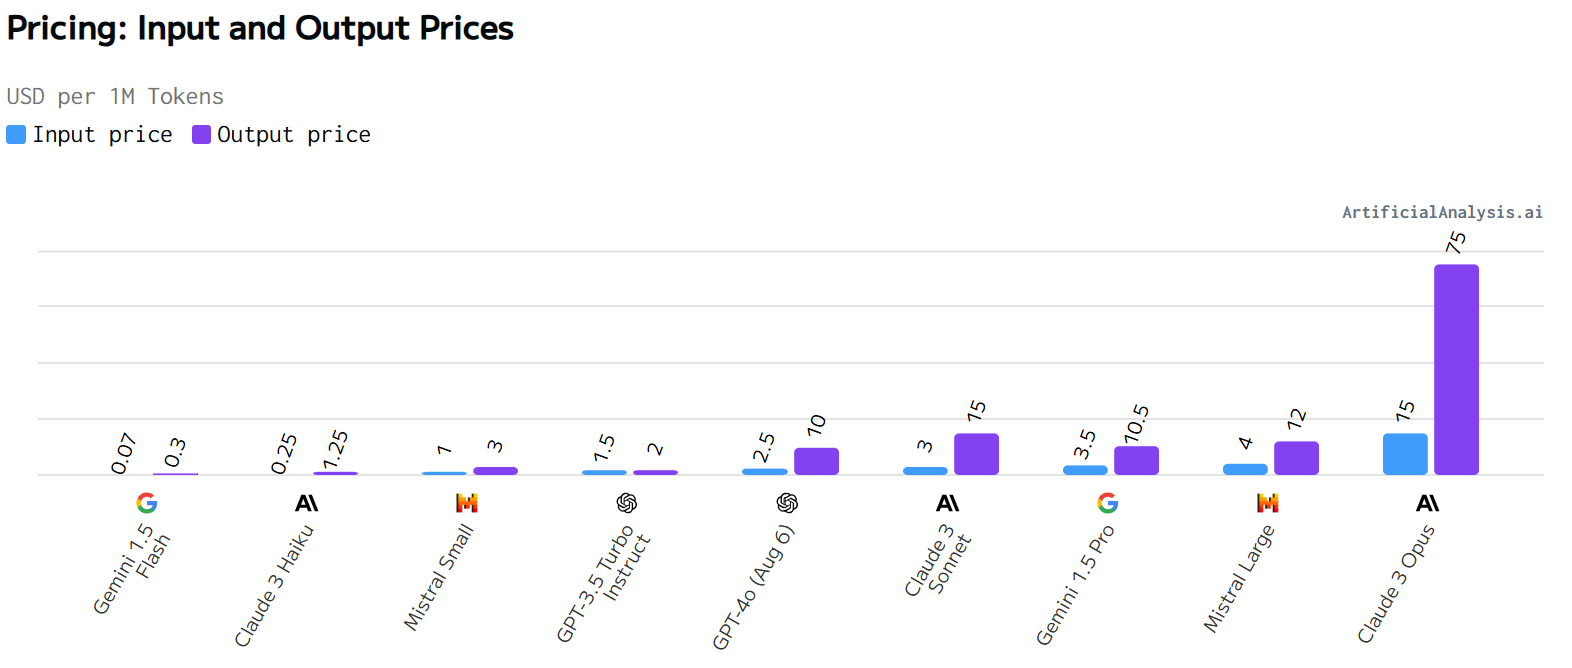
\includegraphics[width=0.9\textwidth]{figuras/capitulo6/pricing.png}
\caption{Benchmark sobre el precio de los LLMs evaluados. \citep{artificialanalysis}}
\label{fig:pricing}
\end{figure}

\begin{figure}[h]
\centering
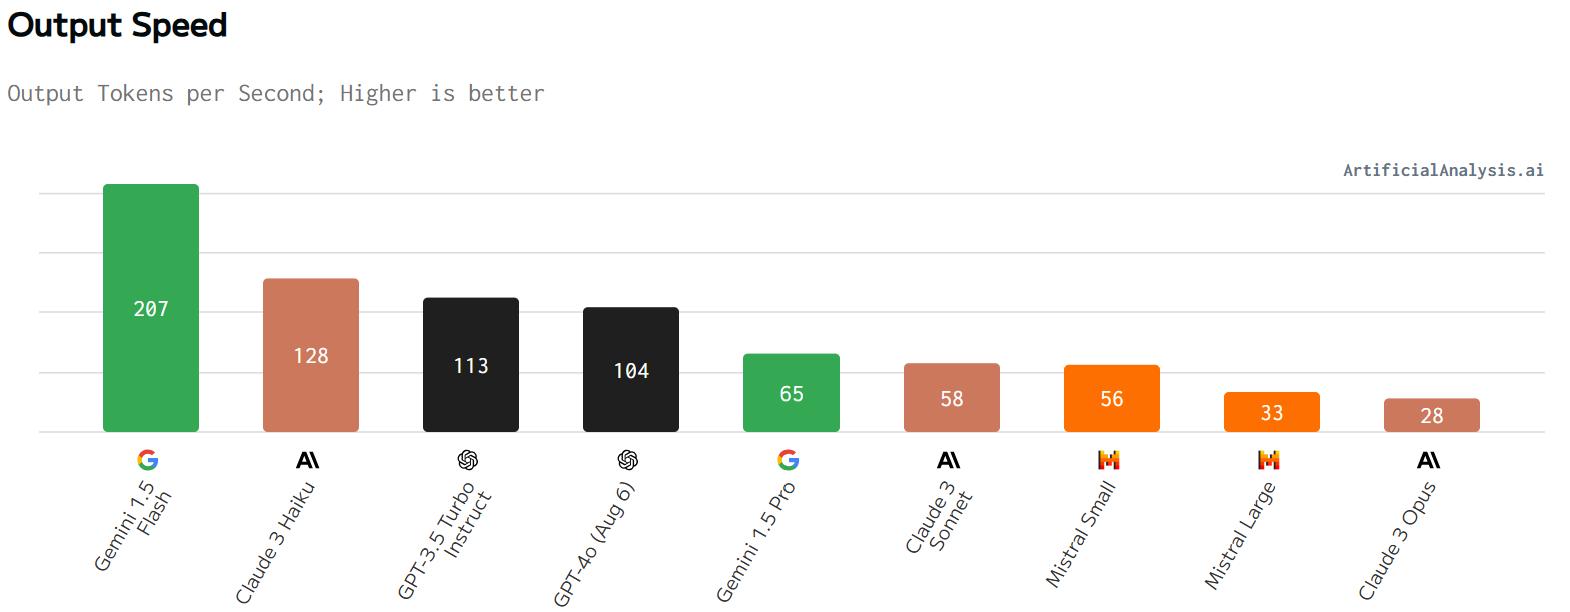
\includegraphics[width=0.9\textwidth]{figuras/capitulo6/speed.png}
\caption{Benchmark sobre la velocidad de respuesta de los LLMs evaluados. \citep{artificialanalysis}}
\label{fig:speed}
\end{figure}

\begin{figure}[]
\centering
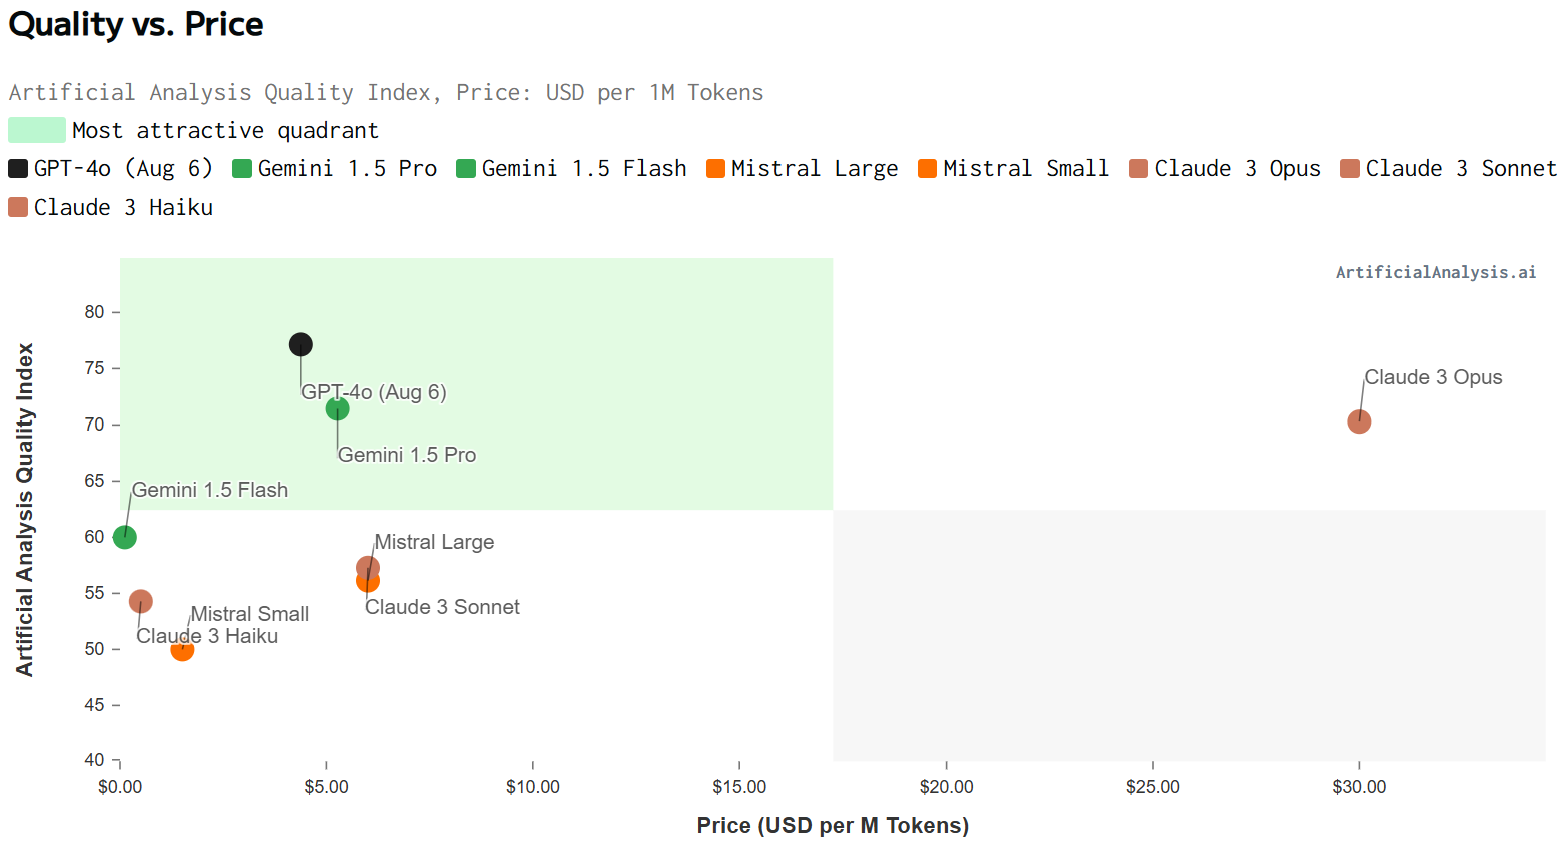
\includegraphics[width=0.9\textwidth]{figuras/capitulo6/quality_price.png}
\caption{Gráfico comparativa calidad contra precio. \citep{artificialanalysis}}
\label{fig:quality_price}
\end{figure}

\subsection{Modelo Embedder}

Este modelo es el encargado de transformar los fragmentos del documento en vectores o embeddings. Este modelo es de alta importancia en el proceso ya que será el que defina la similitud entre los textos. Por tanto es crucial para la recuperación de la información necesaria para dar una respuesta.

El modelo embedder ha sido text-embedding-3-small con posición 59 en el leaderboard de huggingface \citep{leadhugging}. Se ha usado este modelo por ser el mejor calidad/precio disponible en Azure OpenAI. Como se puede ver en la figura \ref{fig:emb_quality} mejora al anterior model ada v2 y se puede ver en la tabla \ref{tab:pricing} como reduce su precio. Por estas dos razones es el modelo seleccionado para el sistema RAG creado.

\begin{figure}[h]
\centering
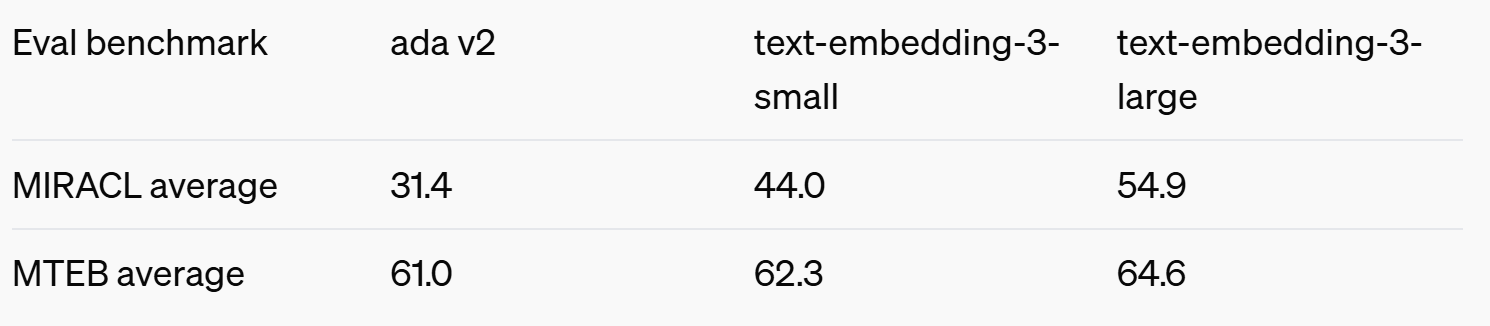
\includegraphics[width=0.9\textwidth]{figuras/capitulo6/emb_quality.png}
\caption{Gráfico calidad embeddings OpenAI \citep{openai}}
\label{fig:emb_quality}
\end{figure}

\begin{table}[h]
\centering
\begin{tabular}{|c|c|}
\hline
\textbf{Model} & \textbf{Pricing} \\ \hline
text-embedding-3-small & \$0.020 / 1M tokens \\ \hline
text-embedding-3-large & \$0.130 / 1M tokens \\ \hline
ada v2 & \$0.100 / 1M tokens \\ \hline
\end{tabular}
\caption{Precio de los embeddings de OpenAI \citep{openai}}
\label{tab:pricing}
\end{table}


\section{Análisis del Documento: Constitución Española}

\subsection{Estructura del Documento}

La \textbf{Constitución Española} es el documento fundamental que establece el marco legal y político de España. Fue ratificada en 1978 y es el texto supremo que rige los derechos, deberes y la organización de las instituciones del país. El documento está dividido en varios títulos que abordan aspectos clave del sistema político, económico y social de España. Se compone de una introducción (Preámbulo) y 10 títulos, además de disposiciones adicionales, transitorias, derogatorias y finales.

\begin{itemize}
    \item \textbf{Preámbulo}: Establece los principios y objetivos fundamentales de la Constitución, como la justicia, la libertad, la democracia, la protección de los derechos humanos, el progreso social y la promoción de la paz y la cooperación internacional.
    \item \textbf{Títulos}:
    \begin{itemize}
        \item \textbf{Título Preliminar}: Define a España como un Estado social y democrático de derecho y establece la soberanía nacional y la forma política del Estado, que es la monarquía parlamentaria.
        \item \textbf{Título I}: Regula los derechos y deberes fundamentales, dividiéndose en varios capítulos que incluyen los derechos de los españoles y los extranjeros, así como las libertades y derechos fundamentales.
        \item \textbf{Título II}: Describe la Corona y las funciones del Rey como jefe de Estado.
        \item \textbf{Títulos III a V}: Tratan sobre las Cortes Generales, el Gobierno y las relaciones entre ambos poderes.
        \item \textbf{Título VI}: Regula el poder judicial.
        \item \textbf{Títulos VII a X}: Abordan la economía y hacienda, la organización territorial del Estado, el Tribunal Constitucional y la reforma constitucional.
    \end{itemize}
\end{itemize}

\subsection{Relevancia para el Sistema RAG}

El \textbf{sistema RAG (Retrieval-Augmented Generation)} que se propone desarrollar utilizará este documento como base de conocimiento para responder preguntas relacionadas con la Constitución Española. Debido a su estructura bien definida y la clara división de temas, es posible fragmentar el documento en secciones más manejables que puedan ser recuperadas de manera eficiente.

\subsection{Formato del documento}

El documento se encuentra tanto en formato PDF como en formato XML. En el formato XML se puede acceder a cada uno de los artículos de la constitución por separado. Se muestra un ejemplo a continuación:

\begin{verbatim}
</div>
<p class="linkSubir"><a href="https://www.boe.es/buscar/act.php?
id=BOE-A-1978-31229&amp;p=20240217&amp;tn=1#top">Subir</a></p>
<hr class="bloque">
<div class="bloque" id="a3">
  <p class="bloque">[Bloque 5: #a3]</p>
  <form action="https://www.boe.es/buscar/act.php?id=BOE-A-1978-31229&amp;
  p=20240217&amp;tn=1#" method="get">
    <input type="hidden" value="BOE-A-1978-31229" name="id">
    <input type="hidden" value="5" name="tn">
    <input type="hidden" value="a3" name="bj">
    <input id="btn_jur_a3" type="submit">
    <label for="btn_jur_a3" title="Jurisprudencia">
      <span class="fuera">Jurisprudencia</span>
    </label>
  </form>
  <h5 class="articulo">Artículo 3</h5>
  <p class="parrafo">1. El castellano es la lengua española oficial del Estado. 
  Todos los españoles tienen el deber de conocerla y el derecho a usarla.</p>
  <p class="parrafo">2. Las demás lenguas españolas serán también oficiales en las 
  respectivas Comunidades Autónomas de acuerdo con sus Estatutos.</p>
  <p class="parrafo">3. La riqueza de las distintas modalidades lingüísticas de 
  España es un patrimonio cultural que será objeto de especial respeto y protección.</p>
</div>
\end{verbatim}

\section{Chunkerización del Documento}

La chunkerización es un proceso crucial en la creación de sistemas de Recuperación Aumentada por Generación (RAG, por sus siglas en inglés). En este capítulo, se describe cómo se realiza la chunkerización del documento de la Constitución Española para mejorar la eficiencia en la recuperación de la información. Utilizamos diferentes estrategias de chunkerización que se adaptan a la naturaleza del texto y el caso de uso. Para implementar estas estrategias, utilizamos la librería \texttt{LangChain}, que ofrece una serie de herramientas avanzadas para manejar documentos de gran tamaño.

\section{Estrategias de Chunkerización}

La chunkerización del documento implica dividir el texto en fragmentos más pequeños y manejables (chunks). Esto mejora la precisión de la recuperación de información al asegurar que los fragmentos estén centrados en temas específicos. A continuación, se explican las tres estrategias de chunkerización empleadas:

\subsection{Character Text Splitter}
El \textit{Character Text Splitter} es una de las técnicas básicas de chunkerización. Divide el texto en fragmentos basándose en un número fijo de caracteres, lo que asegura que los fragmentos resultantes tengan un tamaño consistente. Esta técnica es útil cuando se requiere dividir grandes bloques de texto de manera uniforme, pero no considera la semántica ni la estructura del texto.

Para esta estrategia, definimos tamaños de chunk de 200, 300 y 400 caracteres, con un pequeño solapamiento entre los fragmentos (10 \% del tamaño del chunk), lo que permite preservar el contexto cuando se fragmenta el documento. Este método es sencillo y eficiente para manejar grandes volúmenes de datos.

\subsection{Recursive Character Text Splitter}
El \textit{Recursive Character Text Splitter} es una versión más avanzada del \textit{Character Text Splitter}. Además de dividir el texto basándose en el número de caracteres, este enfoque aplica un análisis recursivo, respetando la estructura del documento al intentar evitar cortar palabras o frases importantes. De esta manera, los fragmentos generados tienen mayor coherencia interna y preservan mejor el contexto semántico, lo que mejora las respuestas generadas en los sistemas RAG.

Al igual que con el splitter básico, se utilizan tamaños de chunk de 200, 300 y 400 caracteres, pero con el beneficio añadido de que los fragmentos resultan más naturales y mejor alineados con las divisiones lógicas del texto.

\subsection{Chunkerización personalizada (Spanish Article Splitter)}
El \textit{Spanish Article Splitter} ha sido desarrollado específicamente para chunkerizar documentos legales en español, como la Constitución Española. Este splitter aprovecha la estructura inherente del documento en XML, basada en artículos, para realizar la chunkerización. Utilizando técnicas de procesamiento de HTML, el splitter identifica los artículos individuales y los divide en fragmentos de texto correspondientes. Cada artículo es tratado como un fragmento separado, preservando su integridad semántica.

Este splitter es particularmente útil en textos legales, donde cada artículo puede ser considerado una unidad independiente y completa de información. Para documentos como la Constitución Española, esta técnica asegura que los fragmentos de texto sean coherentes y estén alineados con la estructura legal del documento.

El pseudocódigo del algoritmo desarrollado se encuentra en el algoritmo \ref{alg:SpanishArticleSplitter}.


\begin{algorithm}
\caption{SpanishArticleSplitter}\label{alg:SpanishArticleSplitter}
\textbf{Entrada:} Ruta del archivo HTML (\textit{file\_path}) \;
\textbf{Salida:} Lista de documentos divididos por artículos (\textit{documents}) \;

Abrir el archivo en la ruta especificada (\textit{file\_path}) y leer su contenido como HTML\;
Parsear el contenido HTML utilizando un parser compatible con HTML\;
Inicializar una lista vacía para almacenar los documentos (\textit{documents})\;
Encontrar todos los elementos de encabezado \texttt{<h5>} con la clase \texttt{articulo}\;
\For{cada \texttt{<h5>} encontrado}{
    Encontrar el \texttt{<div>} que contiene el artículo asociado\;
    Extraer el nombre del artículo desde el texto del encabezado \texttt{<h5>}\;
    Inicializar una lista vacía para los párrafos del artículo\;
    \For{cada párrafo \texttt{<p>} dentro del \texttt{<div>}}{
        \If{el texto del párrafo no contiene \texttt{"Bloque"}}{
            Agregar el texto del párrafo a la lista\;
        }
    }
    Unir todos los párrafos para formar el texto completo del artículo\;
    Crear un diccionario de metadatos con nombre del artículo, nombre del archivo y fuente del archivo\;
    Crear un documento con el texto del artículo y los metadatos\;
    Agregar el documento a la lista \textit{documents}\;
}
Retornar la lista de documentos \textit{documents}\;
\end{algorithm}

\subsection{Librería LangChain}
La librería usada para esta tarea ha sido \texttt{LangChain}. Proporciona una plataforma robusta para la manipulación y chunkerización de documentos. Permite el uso de diferentes tipos de splitters para dividir el texto según las necesidades del usuario. En este caso, se emplearon tanto splitters estándar como personalizados. La flexibilidad de \texttt{LangChain} facilita la integración de diferentes enfoques, desde la división básica de texto por caracteres hasta estrategias más complejas como el \textit{Spanish Article Splitter}.

LangChain también facilita el procesamiento de diferentes formatos de documentos (como PDF y HTML) y su posterior transformación en fragmentos manejables para mejorar la eficiencia en los procesos de recuperación y generación de texto.\\

En total se obtienen 7 formas de fragmentar el documento que deberán ser evaluadas.


\section{Evaluación del sistema RAG}

Para evaluar la efectividad de la chunkerización en el sistema RAG creado, se utilizó un proceso exhaustivo que involucró la generación y evaluación de preguntas basadas en los fragmentos generados de la Constitución Española. Este proceso de evaluación fue realizado utilizando la librería \texttt{LlamaIndex}, que permitió automatizar tanto la generación de preguntas como la medición de métricas clave para determinar la calidad de las respuestas generadas.

Es importante puntualizar que el número de chunks devueltos por el sistema RAG de cara a su evaluación ha sido de 2 chunks.

\subsection{Generación de Preguntas}

El primer paso consistió en generar un conjunto de preguntas para evaluar la precisión y relevancia de las respuestas proporcionadas por el sistema. Para ello, se utilizó el modelo GPT-3.5-turbo, que empleó un \textit{prompt} diseñado para generar preguntas en español a partir de fragmentos de texto extraídos de los documentos chunkerizados. Este conjunto de preguntas se almacenó en un archivo CSV para su posterior uso en la evaluación.

Se usó el siguiente prompt para la generación de preguntas:

\begin{verbatim}
Context information is below.
---------------------
{context_str}
---------------------
Given the context information and not prior knowledge,
generate only questions based on the below query.
Generate the questions in Spanish.
{query_str}
\end{verbatim}

\begin{table}[h]
\centering
\begin{tabular}{|c|}
\hline
\textbf{Questions} \\ \hline
¿Cuáles son los valores superiores del ordenamiento jurídico en España? \\ \hline
¿En quién reside la soberanía nacional en España? \\ \hline
¿Cuál es la forma política del Estado español? \\ \hline
¿Cómo se define a España en términos de su Estado? \\ \hline
¿Cuáles son los principios fundamentales de España como Estado? \\ \hline
¿Cuál es el sistema político de España? \\ \hline
¿Qué poderes emanan del pueblo español? \\ \hline
¿Qué tipo de monarquía tiene España? \\ \hline
... \\ \hline
\end{tabular}
\caption{Ejemplo de preguntas generadas}
\label{tab:questions}
\end{table}


\subsection{Métricas de Evaluación}

Las métricas de evaluación clave empleadas en este proceso se centran en tres aspectos fundamentales para sistemas RAG: fidelidad, relevancia de la respuesta, relevancia del contexto y tiempo de respuesta. Estas métricas se calcularon utilizando el modelo GPT-4o (\textbf{modelo juez}), que permitió evaluar de manera automática la calidad de las respuestas generadas para cada pregunta.

\begin{itemize}
    \item \textbf{Fidelidad (FP)}: Mide hasta qué punto las respuestas generadas están respaldadas por el contexto proporcionado. Es decir, se asegura de que las afirmaciones hechas en las respuestas sean consistentes con la información del documento original, minimizando la aparición de alucinaciones. En la implementación de LlamaIndex el resultado será True o False.
    \item \textbf{Relevancia de la Respuesta (RP)}: Evalúa si la respuesta aborda directamente la pregunta formulada. Este criterio no solo considera la factualidad, sino también si la respuesta es completa y libre de información redundante o innecesaria. En la implementación de LlamaIndex el resultado será True o False.
    \item \textbf{Relevancia del Contexto (RCP)}: Mide cuán relevante es el contexto recuperado para responder la pregunta. Un buen contexto debe contener únicamente la información necesaria para proporcionar una respuesta precisa, sin añadir detalles irrelevantes que puedan afectar la calidad de la generación de texto.
    \item \textbf{Tiempo de respuesta (TRP)}: El tiempo en el que el sistema RAG completo da una respuesta a la pregunta del usuario.
\end{itemize}

Cabe recalcar que ninguna de las métricas usadas necesita la respuesta verdadera a la pregunta ya que analizan la respuesta en base al contexto (los chunks) aportado.

En la tabla \ref{tab:evaluation1} puede verse un ejemplo de error con la respuesta, sin embargo todas las métricas cumplen su función.

\begin{itemize}
    \item \textbf{Fidelidad}: El resultado es True ya que no hay alucinación en la respuesta. El Agente LLM no tiene en el contexto la información que el usuario solicita por lo que la respuesta es correcta al responder que no puede responder.
    \item \textbf{Relevancia de la Respuesta}: Esta métrica mide la relevancia de la respuesta a la pregunta. En otras palabras si responde la pregunta del usuario. El resultado es True, ya que responde que no puede responder con la información que tiene, pero responde a la pregunta formulada.
    \item \textbf{Relevancia del Contexto}: En esta métrica si podemos comprobar que el contexto no es el adecuado para responder a la pregunta y el modelo juez aporta la explicación de esta métrica.
\end{itemize}

\begin{table}[h]
\centering
\begin{tabular}{|p{4cm}|p{11cm}|}
\hline
\textbf{Field} & \textbf{Content} \\ \hline
\textbf{Question} & ¿Cuál es el contenido del artículo 28 de la Constitución Española? \\ \hline
\textbf{Response} & El contenido del artículo 28 de la Constitución Española no se encuentra proporcionado en el contexto dado. \\ \hline
\textbf{Context 1} & 
\textbf{Article Name:} Artículo 53 \newline 
\textbf{Text:} Los derechos y libertades reconocidos en el Capítulo segundo del presente Título vinculan a todos los poderes públicos... \newline
\textbf{Source:} ../data/Constitución Española/BOE-A-1978-31229 Constitución Española.html
\\ \hline
\textbf{Context 2} & 
\textbf{Article Name:} Artículo 20 \newline
\textbf{Text:} Se reconocen y protegen los derechos: \newline
a) A expresar y difundir libremente los pensamientos, ideas y opiniones mediante la palabra, el escrito o cualquier otro medio... \newline
\textbf{Source:} ../data/Constitución Española/BOE-A-1978-31229 Constitución Española.html
\\ \hline
\textbf{Faithfulness} & True \\ \hline
\textbf{Relevancy} & True \\ \hline
\textbf{Context Relevancy Score} & 0.125 \\ \hline
\textbf{Context Relevancy Feedback} & 
\textbf{Feedback:} \newline
- The context is related to the Spanish Constitution but does not specifically match Article 28. \newline
- **Score:** 0.5/2 \newline
- The context does not provide the specific content needed to answer the query. \newline
- **Final Score:** 0.5
\\ \hline
\textbf{Response Time} & 1.253065586090088 seconds \\ \hline
\end{tabular}
\caption{Ejemplo evaluación pregunta 1}
\label{tab:evaluation1}
\end{table}

\begin{table}[h]
\centering
\begin{tabular}{|p{4cm}|p{11cm}|}
\hline
\textbf{Field} & \textbf{Content} \\ \hline
\textbf{Question} & ¿Cuál es el objetivo de la educación según los principios constitucionales? \\ \hline
\textbf{Response} & El objetivo de la educación según los principios constitucionales es el pleno desarrollo de la personalidad humana en el respeto a los principios democráticos de convivencia y a los derechos y libertades fundamentales. \\ \hline
\textbf{Context 1} & 
\textbf{Article Name:} Artículo 27 \newline 
\textbf{Text:} Todos tienen el derecho a la educación. Se reconoce la libertad de enseñanza... \newline
\textbf{Source:} ../data/Constitución Española/BOE-A-1978-31229 Constitución Española.html
\\ \hline
\textbf{Context 2} & 
\textbf{Article Name:} Artículo 9 \newline
\textbf{Text:} Los ciudadanos y los poderes públicos están sujetos a la Constitución... \newline
\textbf{Source:} ../data/Constitución Española/BOE-A-1978-31229 Constitución Española.html
\\ \hline
\textbf{Faithfulness} & True \\ \hline
\textbf{Relevancy} & True \\ \hline
\textbf{Context Relevancy Score} & 1.0 \\ \hline
\textbf{Context Relevancy Feedback} & 
\textbf{Feedback:} \newline
- The retrieved context directly addresses the query about the objective of education. \newline
- **Score:** 2/2 \newline
- The context can be used exclusively to fully answer the query. \newline
- **Final Score:** 4.0
\\ \hline
\textbf{Response Time} & 2.0108368396759033 seconds \\ \hline
\end{tabular}
\caption{Ejemplo evaluación pregunta 2}
\label{tab:evaluation12}
\end{table}

\subsection{Evaluación}

Se creó una base de datos vectorial sobre chroma utilizando los grupos de documentos chunkerizados anteriormente, y para cada pregunta y grupo de chunks (cada metodología de chunkerización descrita), el sistema calculó las métricas de fidelidad, relevancia de la respuesta, relevancia del contexto y tiempo de respuesta.

El proceso de evaluación se llevó a cabo mediante la generación de respuestas automáticas a las preguntas formuladas. Se calculó el promedio de las métricas para cada metodología de chunks. Finalmente, los resultados de las métricas se almacenaron en un archivo JSON para su análisis posterior.

\subsection{Resultados}

Se presentan los resultados de la evaluación de diferentes técnicas de chunkerización aplicadas al sistema RAG. A continuación, se describen los resultados obtenidos para cada estrategia de chunkerización (véase tabla \ref{tab:chunk_results} y la figura \ref{fig:chunk_plot}):

\begin{itemize}
    \item \textbf{Spanish Article Splitter}: Esta estrategia produjo un tiempo de respuesta promedio de 1.56 segundos, con una fidelidad promedio de 0.94, una relevancia promedio de 0.94 y una relevancia del contexto de 0.86. Estos resultados muestran que este splitter mantiene un alto nivel de precisión en las respuestas y una relevancia adecuada del contexto, aunque el tiempo de respuesta es ligeramente superior a otras estrategias.
    
    \item \textbf{Character Splitter (400 caracteres)}: El tiempo de respuesta promedio fue de 1.52 segundos, con una fidelidad de 0.95, relevancia de 0.91 y relevancia del contexto de 0.72. Esta estrategia proporcionó un excelente balance entre fidelidad y relevancia, aunque la relevancia del contexto es menor en comparación con el splitter basado en artículos.
    
    \item \textbf{Recursive Character Splitter (400 caracteres)}: Este splitter alcanzó un tiempo de respuesta promedio de 1.50 segundos, con una fidelidad de 0.93, relevancia de 0.87 y relevancia del contexto de 0.69. Aunque la relevancia del contexto es menor, esta técnica ofrece un buen equilibrio entre tiempos de respuesta y precisión.
    
    \item \textbf{Recursive Character Splitter (200 caracteres)}: El tiempo de respuesta promedio fue el más bajo con 1.43 segundos. La fidelidad promedio fue de 0.95, la relevancia de 0.85 y la relevancia del contexto de 0.65. Aunque presenta buenos tiempos de respuesta, la relevancia del contexto es la más baja entre las estrategias evaluadas.
    
    \item \textbf{Character Splitter (300 caracteres)}: Con un tiempo de respuesta promedio de 1.30 segundos, esta estrategia obtuvo una fidelidad de 0.91, relevancia de 0.83 y relevancia del contexto de 0.67. Aunque el tiempo de respuesta es rápido, las métricas de relevancia están ligeramente por debajo de otras técnicas.
    
    \item \textbf{Recursive Character Splitter (300 caracteres)}: Este splitter alcanzó un tiempo de respuesta promedio de 1.39 segundos, con una fidelidad de 0.94, relevancia de 0.90 y relevancia del contexto de 0.69. Aunque el tiempo de respuesta es mayor que otras técnicas, ofrece un buen compromiso entre precisión y relevancia de las respuestas.
    
    \item \textbf{Character Splitter (200 caracteres)}: El tiempo de respuesta promedio fue de 1.36 segundos, con una fidelidad de 0.91, relevancia de 0.82 y relevancia del contexto de 0.65. Este splitter tuvo uno de los tiempos de respuesta más rápidos, pero mostró una ligera disminución en las métricas de relevancia y contexto.

\end{itemize}

En general, los resultados muestran que la estrategia \textit{Spanish Article Splitter} ofrece las mejores métricas de fidelidad y relevancia, a pesar de un tiempo de respuesta ligeramente superior. Por otro lado, las estrategias basadas en \textit{Character Splitter} y \textit{Recursive Character Splitter} presentan una relación equilibrada entre tiempos de respuesta rápidos y métricas de calidad aceptables, con la versión de 400 caracteres proporcionando el mejor compromiso entre velocidad y precisión.

\begin{table}[h]
\centering
\begin{tabular}{|l|c|c|c|c|}
\hline
\textbf{Chunkerización} & \textbf{TRP (s)} & \textbf{FP} & \textbf{RP} & \textbf{RCP} \\ \hline
\textbf{Spanish Article Splitter} & 1.56 & 0.94 & 0.94 & 0.86 \\ \hline
\textbf{Character Splitter (400 caracteres)} & 1.52 & 0.95 & 0.91 & 0.72 \\ \hline
\textbf{Recursive Character Splitter (400 caracteres)} & 1.50 & 0.93 & 0.87 & 0.69 \\ \hline
\textbf{Recursive Character Splitter (200 caracteres)} & 1.43 & 0.95 & 0.85 & 0.65 \\ \hline
\textbf{Character Splitter (300 caracteres)} & 1.30 & 0.91 & 0.83 & 0.67 \\ \hline
\textbf{Recursive Character Splitter (300 caracteres)} & 1.39 & 0.94 & 0.90 & 0.69 \\ \hline
\textbf{Character Splitter (200 caracteres)} & 1.36 & 0.91 & 0.82 & 0.65 \\ \hline
\end{tabular}
\caption{Resultados de la Evaluación de las Técnicas de Chunkerización}
\label{tab:chunk_results}
\end{table}

\begin{figure}[h]
\centering
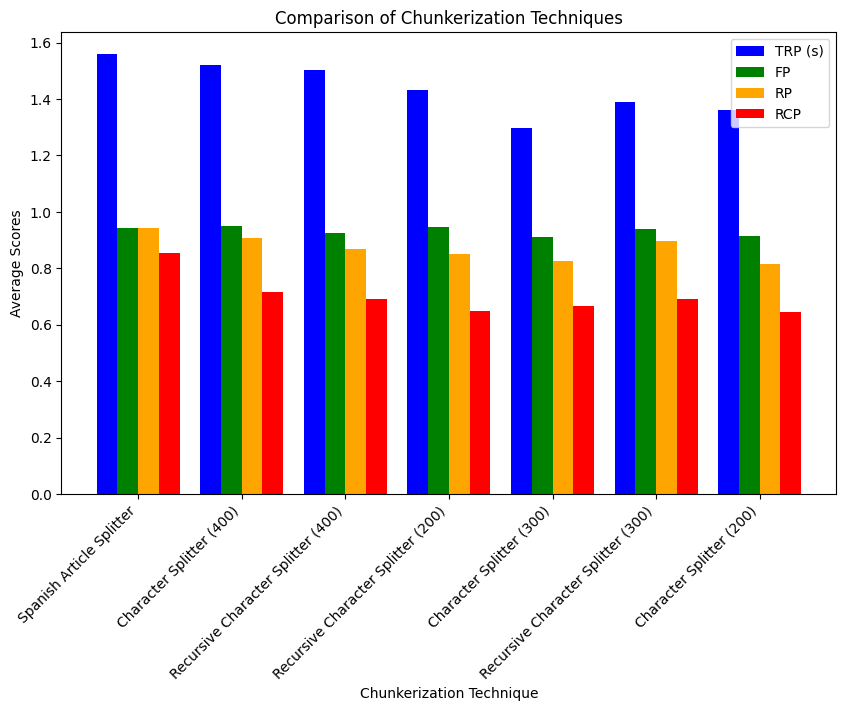
\includegraphics[width=0.6\textwidth]{figuras/capitulo6/score_splitters.png}
\caption{Gráfico comparativo de los splitters evaluados}\label{fig:chunk_plot}
\end{figure}



\section{Creación del agente}

Por último, se ha creado el agente mendiante la librería Langchain usando el splitter personalizado para los artículos de la constitución española. Para ello se ha usado un retriever denso descrito en el capítulo 5. Se ha implementado la arquitectura de la figura \ref{fig:retriever}.

Para que sea más visual (figura \ref{fig:chat1}) y haya una interfaz con la que interactuar con el agente, se ha implementado una app usando la librería Streamlit. En esta interfaz web se pueden hacer preguntas de todo tipo. A continuación se muestran ejemplos de preguntas sobre la interfaz, donde a la vez de ser visualmente más agradable también se muestra un desplegable con el contexto (figura \ref{fig:chat2}) utilizado para responder a la pregunta.

\begin{figure}[h]
\centering
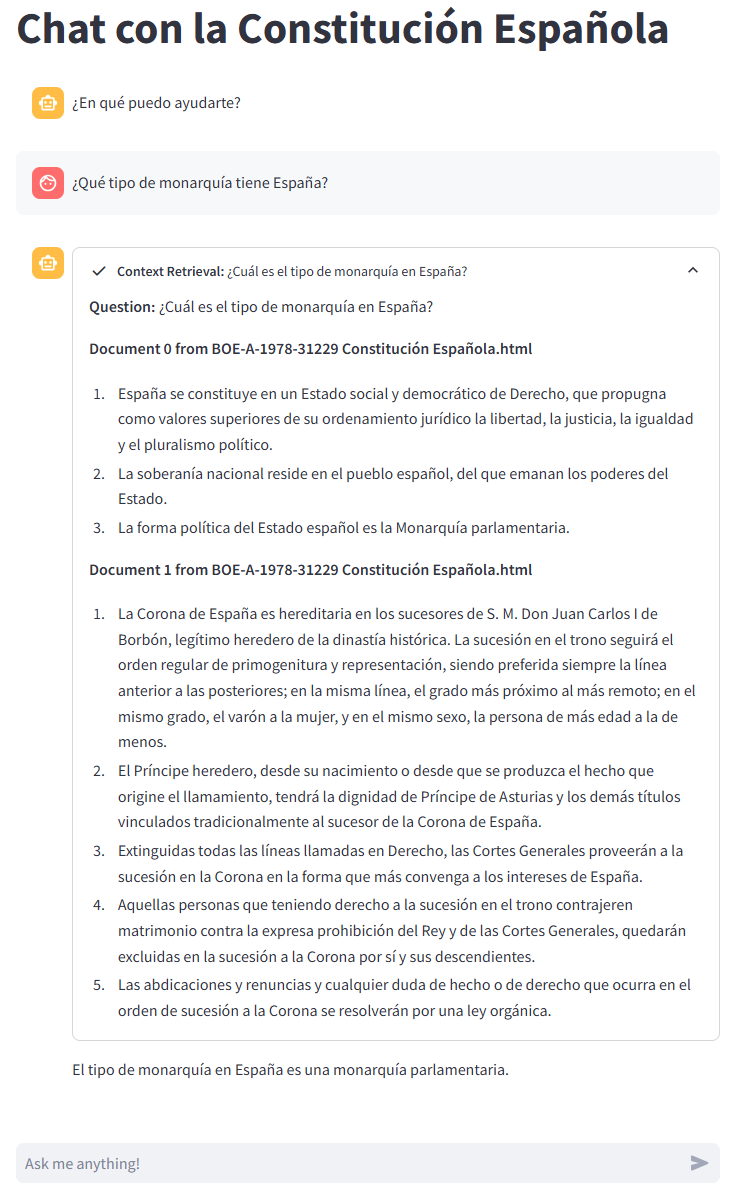
\includegraphics[width=0.7\textwidth]{figuras/capitulo6/chat2exp.png}
\caption{Ejemplo de pregunta en Chat con contexto expandido}\label{fig:chat2}
\end{figure}

\newpage

\begin{figure}[h]
\centering
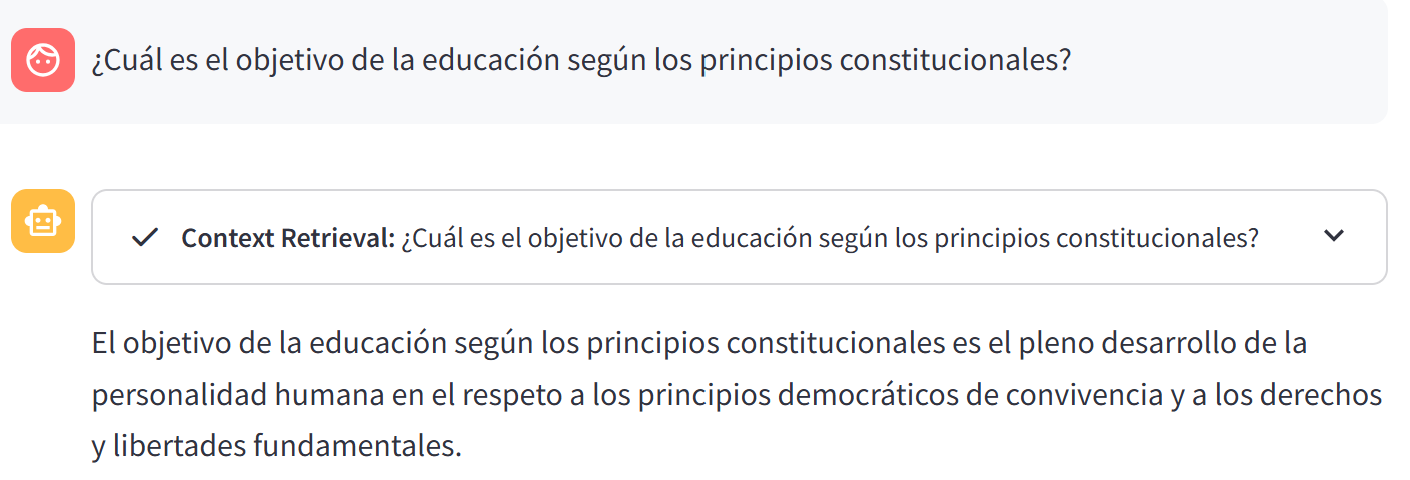
\includegraphics[width=0.7\textwidth]{figuras/capitulo6/chat1.png}
\caption{Ejemplo de pregunta en Chat}\label{fig:chat1}
\end{figure}

\subsection{Diagrama Arquitectura}

El diagrama de arquitectura de la app desarrollada es el siguiente:

\begin{figure}[h]
\centering
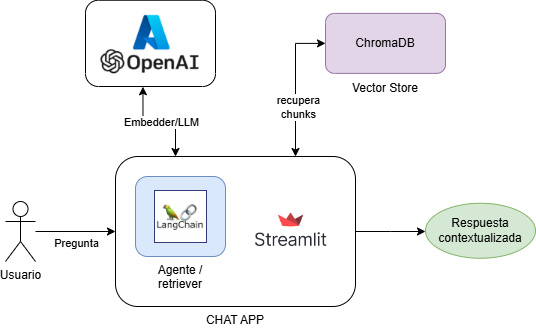
\includegraphics[width=0.7\textwidth]{figuras/capitulo6/arquitectura.png}
\caption{Arquitectura desarrollada}\label{fig:arquitectura}
\end{figure}

En el diagrama se puede ver como las consultas al LLM y al embedder se hacen a través de Azure OpenAI, el vector store utilizado es una instancia de ChromaDB, el agente (retriever) se desarrolla usando el framework Langchain y finalmente la interfaz se ha creado con Streamlit.

\section{Conclusión}

Este capítulo describe la implementación de un sistema RAG para responder preguntas sobre la Constitución Española. Se utilizan modelos LLM como GPT-4o para la evaluación y GPT-3.5-Turbo para generar respuestas, junto con un modelo de embeddings para procesar el texto. Se analizan y prueban varias estrategias de chunkerización del documento, como Character Text Splitter y Spanish Article Splitter, optimizando la recuperación de información.

La evaluación de las técnicas demuestra que el Spanish Article Splitter ofrece la mejor precisión y relevancia del contexto, aunque con un ligero aumento en el tiempo de respuesta. Finalmente, se implementa una interfaz web interactiva para facilitar el uso del sistema, mostrando cómo se puede automatizar la consulta legal de manera eficiente.



%% RESULTADOS Y DISCUSION 

\cleardoublepage

\chapter{Resultados y Discusión}
\label{resultados-y-discusion}

% CONCLUSIONES

\chapter{Conclusiones}
\label{conclusiones}

\begin{enumerate}[label=\destacado{\arabic*.}]
  \setlength\itemsep{1em}
  \item Conclusión 1.

  \item Conclusión 2.

  \item Conclusión 3.
\end{enumerate}

% LIMITACIONES Y PERSPECTIVAS DE FUTURO

\cleardoublepage

\chapter{Limitaciones y\\ Perspectivas de Futuro}
\label{limitaciones-y-futuro}


\cleardoublepage
\phantomsection

\appendix
% APÉNDIZES

% Escribe cada apéndize como si fuera un capítulo más.

\chapter{Apéndize A}
\label{apendize-a}

Figura relativa al benchmark de LLMs.

\begin{figure}[!h]
\centering
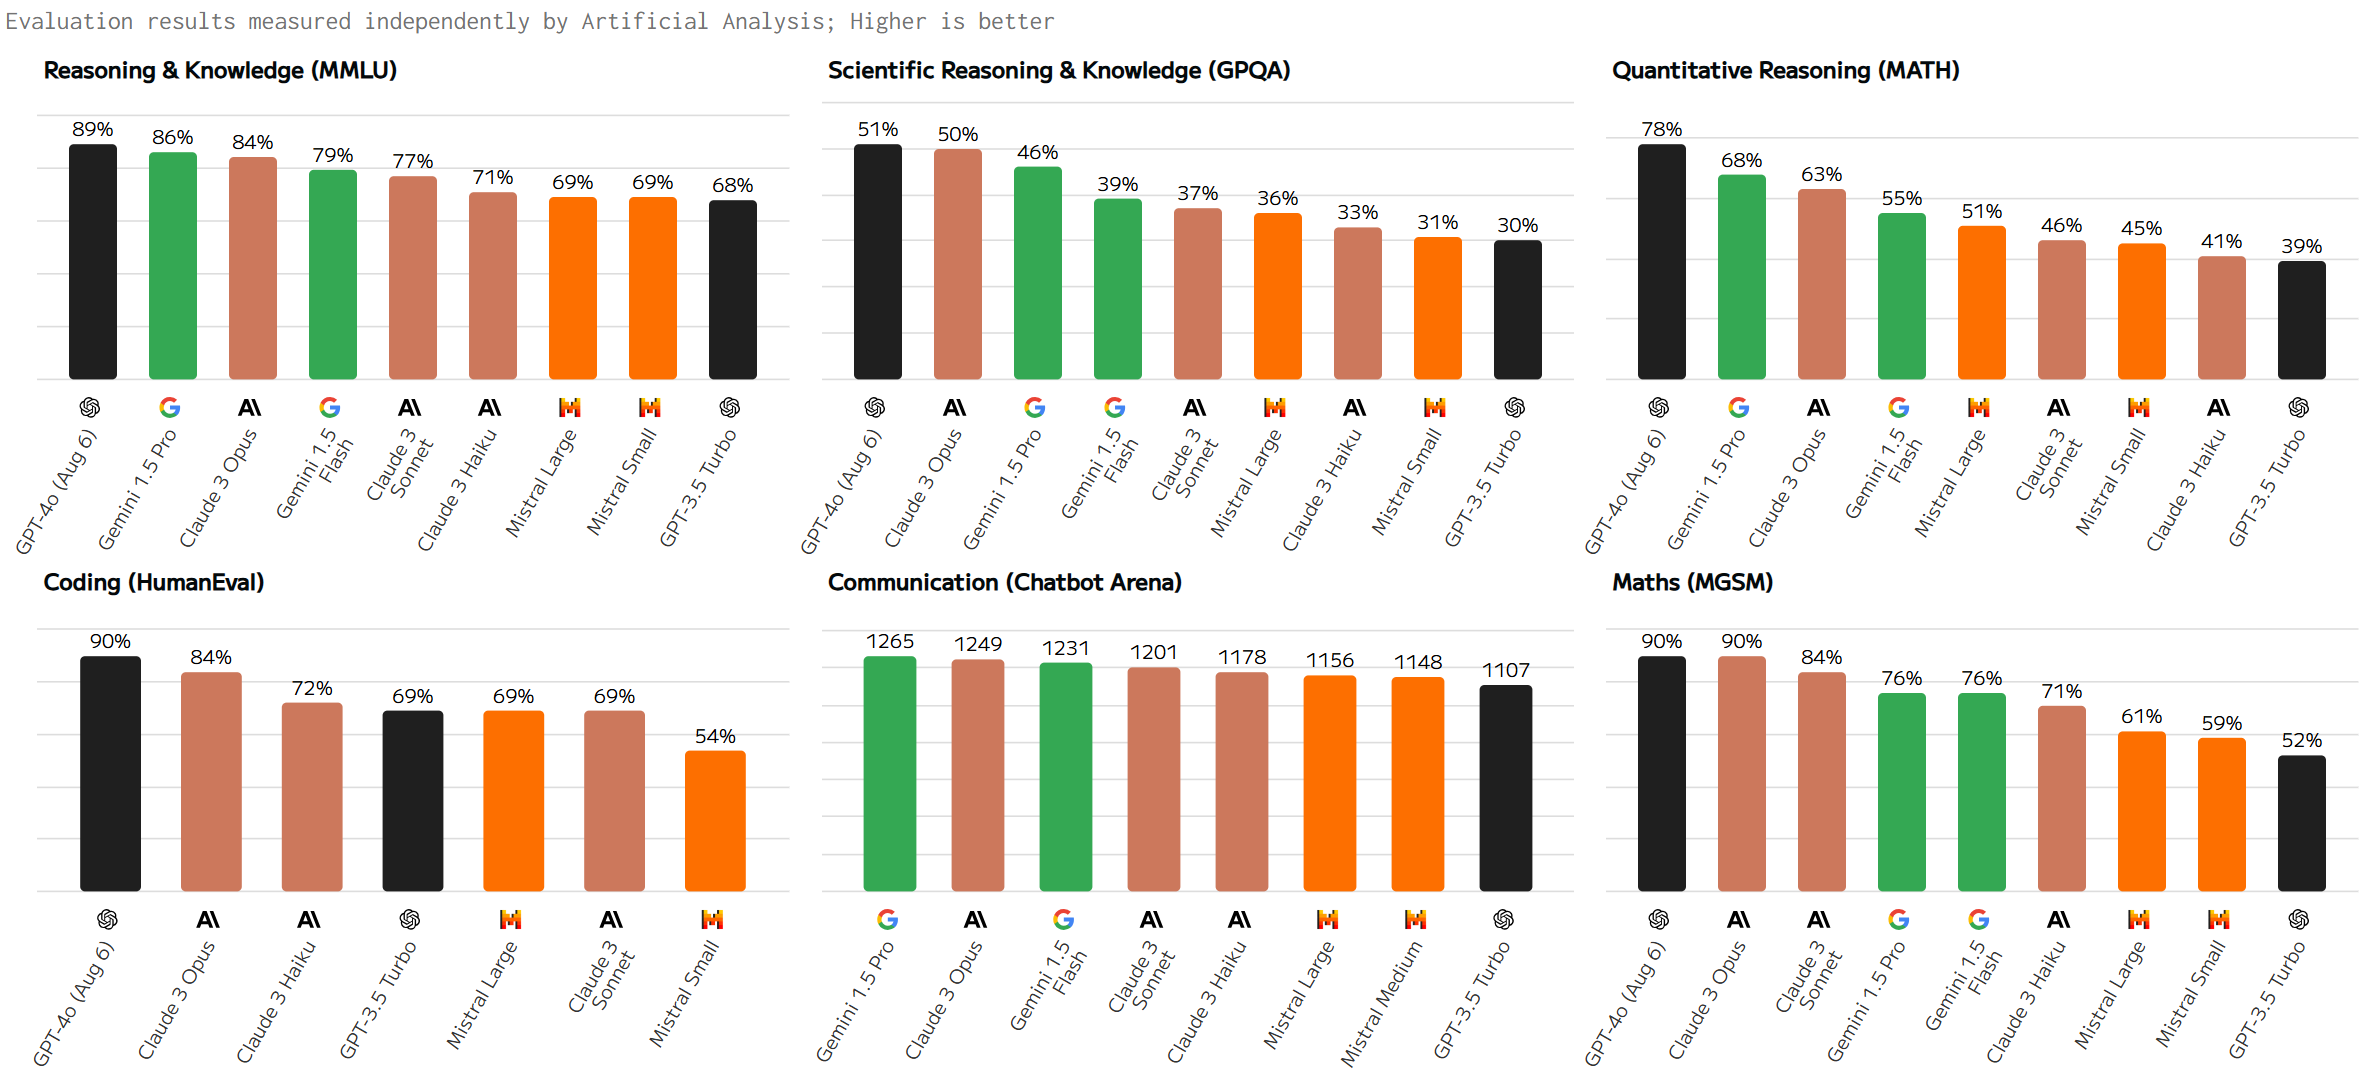
\includegraphics[width=1.1\textwidth,angle=90]{figuras/capitulo6/benchmark.png}
\caption{Benchmark sobre distintas métricas para evaluar LLMs. \citep{artificialanalysis}}
\label{fig:benchmark}
\end{figure}


\begin{singlespace}
\begin{footnotesize}
\begin{twocolumn}
\bibdata{bibliografia}
\bibliography{bibliografia}
\addcontentsline{toc}{chapter}{Bibliografía}
\end{twocolumn}
\end{footnotesize}
\end{singlespace}

\end{document}
